\chapter{Design}
\label{sec:design}

% Ist das zentrale Kapitel der Arbeit. Hier werden das Ziel sowie die
% eigenen Ideen, Wertungen, Entwurfsentscheidungen vorgebracht. Es kann
% sich lohnen, verschiedene Möglichkeiten durchzuspielen und dann
% explizit zu begründen, warum man sich für eine bestimmte entschieden
% hat. Dieses Kapitel sollte - zumindest in Stichworten - schon bei den
% ersten Festlegungen eines Entwurfs skizziert werden.
% Es wird sich aber in einer normal verlaufenden
% Arbeit dauernd etwas daran ändern. Das Kapitel darf nicht zu
% detailliert werden, sonst langweilt sich der Leser. Es ist sehr
% wichtig, das richtige Abstraktionsniveau zu finden. Beim Verfassen
% sollte man auf die Wiederverwendbarkeit des Textes achten.

% Plant man eine Veröffentlichung aus der Arbeit zu machen, können von
% diesem Kapitel Teile genommen werden. Das Kapitel wird in der Regel
% wohl mindestens 8 Seiten haben, mehr als 20 können ein Hinweis darauf
% sein, daß das Abstraktionsniveau verfehlt wurde.

%\ldots design \ldots

%\todo{write design}
This chapter presents a design proposal for a shielding interface that protects applications from being compromised by the OCI interface. Our discussion revolves around the design's various components, functions, interactions, and security 
implications. Our proposed design includes the following parts:

\textbf{Remote attestation and secret provisioning Infrastructure.} This infrastructure forms the cornerstone of secure application deployment and operation by ensuring proper application launch and safeguarding the integrity and confidentiality of 
secrets provisioned by the application owner. Secrets management and deployment are offloaded from Kubernetes and Quark Shim to a trusted relying party. The shield relies on this infrastructure to measure the application launch process and 
establish secure communication with the relying party for secret retrieval.

\textbf{A new pattern for EXEC requests.} This pattern is designed to address three security concerns, namely issuing unauthorized commands to the application, unrestricted allocation of a terminal using kubectl exec -it, and lack of protection for 
commands issued by the application owner. We will explain this further in Section 3.2.
 

\textbf{A mechanism for protecting guest processes' stdio.} This mechanism ensures the protection of the confidentiality and integrity of application logs and terminal data streams belonging to the application owner and prevents attackers from stealing 
the execution results of privileged commands.

\textbf{System call interception.} A user-configurable guest system call interception policy.

\textbf{Qkenrell Log management.} A user-configurable guest logging protection policy.

In the following sections, we first describe the remote attestation and provisioning infrastructure in Section 4.1. We then introduce the new pattern of EXEC requests, the mechanism for protecting the standard IO of guest processes, the guest 
system call interceptor, and the guest log management policy in Sections 4.2, 4.3, 4.4, and 4.5, respectively. Finally, we propose modifications to the OCI interface in Section 4.6.


\section{General Architecture}
The secure virtual machine provides a trusted execution environment that encapsulates the guest, including the Qkernel and application. This environment is also known as an enclave. However, since the Qkernel uses the Qcall, Ucall, and Hcall 
interface to access host services, the shielding layer is added to the Qkernel to prevent attackers from exploiting these interfaces to launch attacks on the enclave. The shield layer controls the communication between the Qkernel and untrusted 
hosts via Ucall, Qcall, and Hcall, modifying the communication according to the shield policy set by the application owner. As this shielding layer is part of the Qkernel, its state is protected by the secure virtual machine.

\begin{figure}[H]
    \centering
    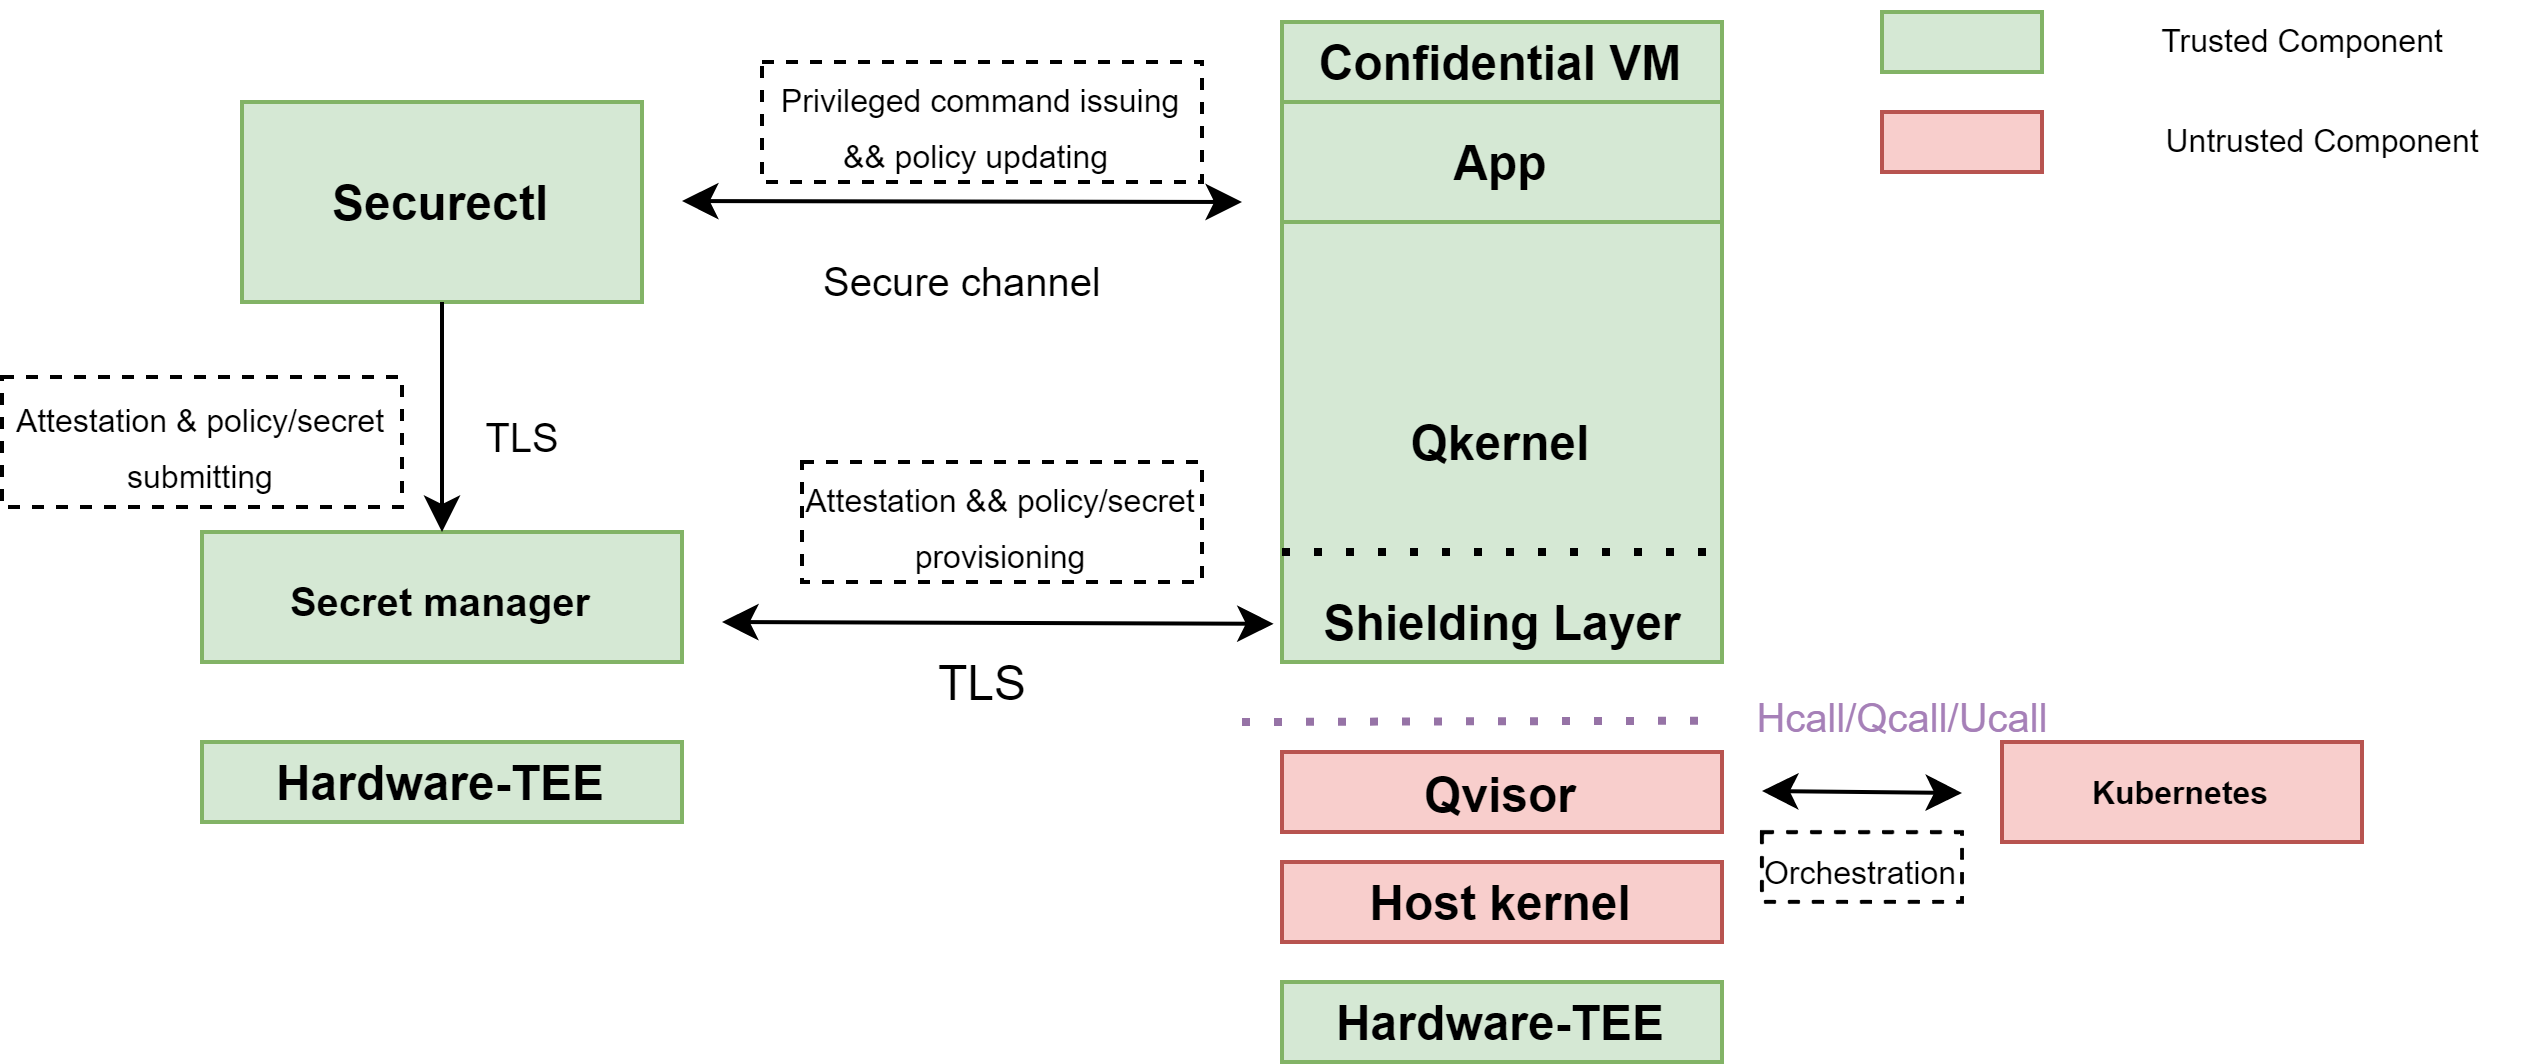
\includegraphics[width=0.8\textwidth]{images/genaral_architechture.png}
    \caption[General Architecture]{General Architecture. The green components in the figure are trusted ,and the red components are not trusted.}
    \label{fig:genaral_architechture}
\end{figure}


On the application owner's side, we introduce Securectl, which establishes a secure channel between the application owner and the enclave. The tool runs in an environment trusted by the application owner and provides an interface to communicate 
with the application and control the shield. The secret manager manages the application's secrets and runs in the cloud, protected by a secure virtual machine. The application owner can authenticate the secret manager using the remote attestation 
mechanism and then upload the secrets through a secure channel. The secret manager validates the application startup process against the policy uploaded by the application owner and securely sends the secrets to the shield. The shield is responsible 
for secret deployment and ensures that the secret is not compromised while the application runs.

\section{Quark Attestation and Provisioning Infrastructure}
This section presents the Quark attestation and provisioning infrastructure, which is designed to facilitate secure application deployment and provides a means for applications to obtain attestation reports at runtime. In particular, it offers mitigation for the following three security issues identified in the security analysis:

Untrusted Kubernetes and Quark-shim manage and deploy applications' secrets.
Corrupted application binaries may be loaded during the application build process.
Lack of measurement of Qkernel command line parameters.

\subsection{Overview}
\begin{figure}[H]
    \centering
    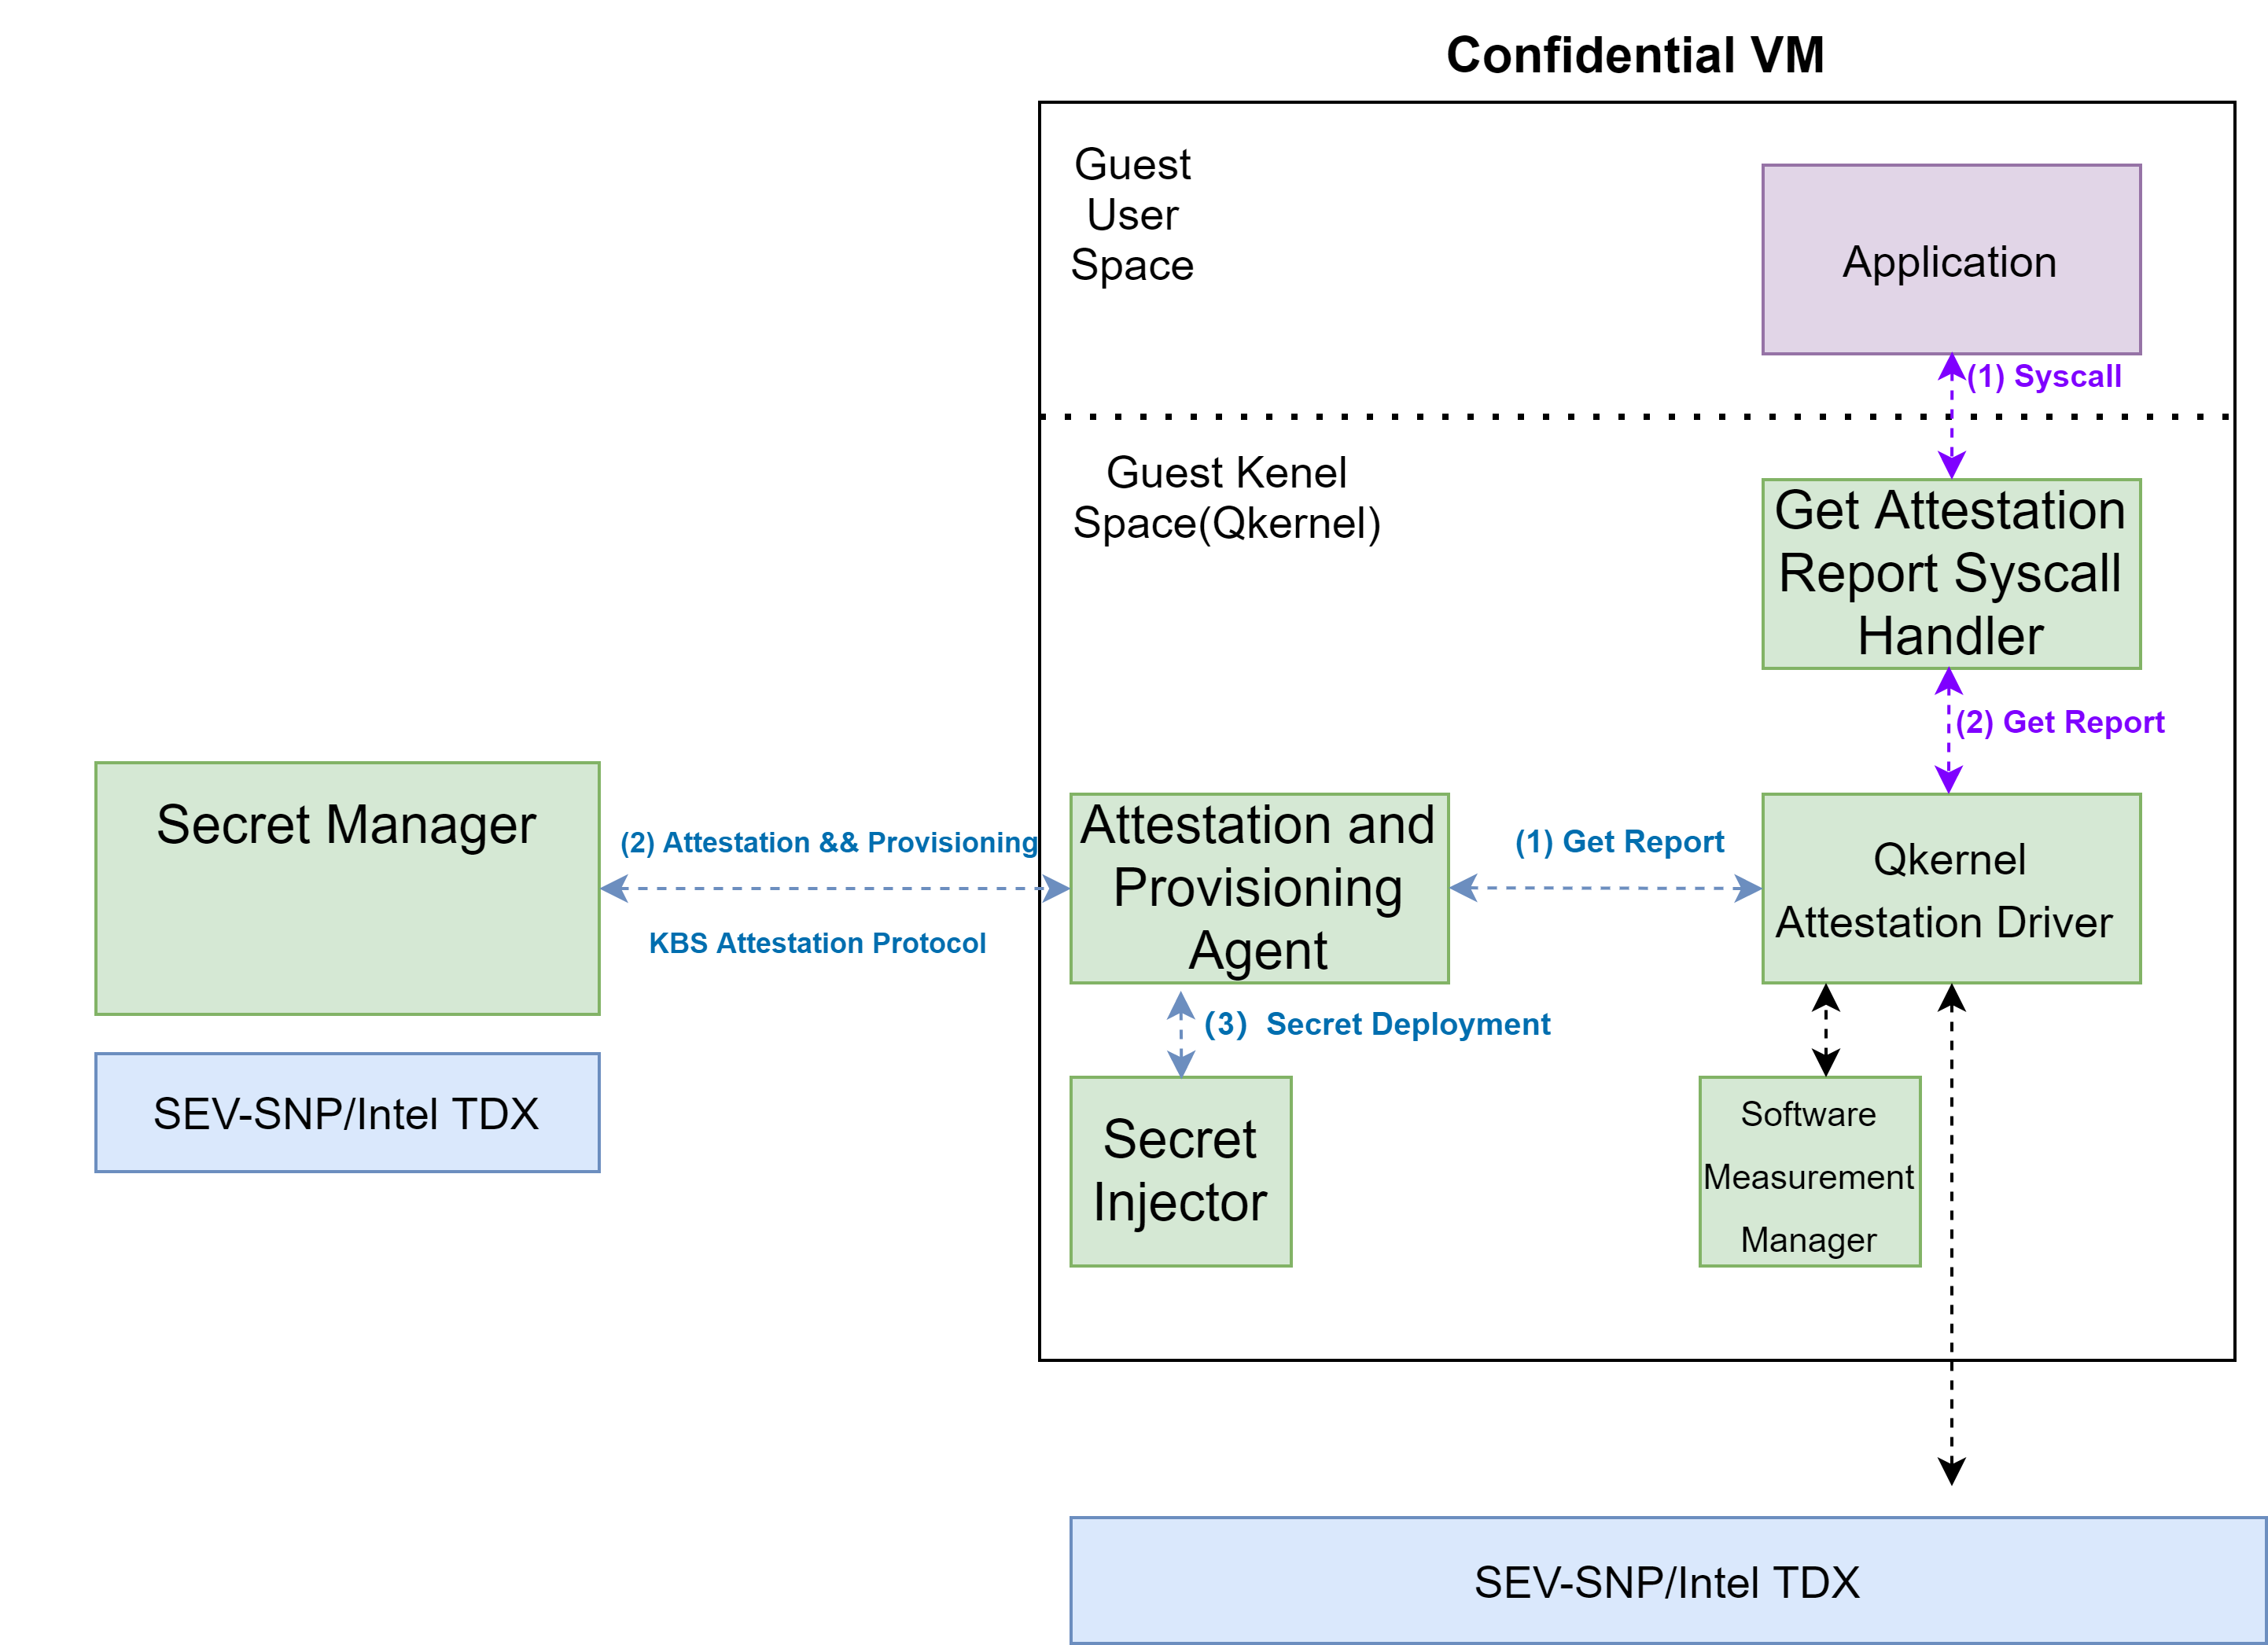
\includegraphics[width=0.8\textwidth]{images/Qkernel_attestation_infrastructurc.png}
    \caption[Quark Attestation and Provisioning Infrastructure]{Quark Attestation and Provisioning Infrastructure}
    \label{fig:Qkernel_attestation_infrastructurc}
\end{figure}

The management and deployment of application secrets are delegated from Kubernetes to the Quark attestation and provisioning infrastructure, as illustrated in Figure~\ref{fig:Qkernel_attestation_infrastructurc}. The infrastructure comprises two 
parts- the secret manager and several components in the enclave shielding layer. These components include the remote attestation and provisioning agent, the secret injector, the Qkernel attestation driver, and the software measurement manager.

The secret manager is responsible for managing and provisioning secrets to the enclave. It runs in a cloud-based trusted execution environment. This guarantees the confidentiality of its managed secrets. The application owner validates the secret 
manager before securely uploading secrets to it. The secrets include the shielding layer's policy, the application's startup parameters, environment variables, and files. The cluster administrator deploys applications. The software measurement 
manager will measure the application binaries and Qkernel startup parameters to ensure correct deployment. The results are sent to the secret manager as part of the enclave's attestation report for integrity check. The report is generated by TEE 
hardware with the help of the Qkernel attestation driver.

During remote attestation and provisioning, the remote attestation and provisioning agent prove its identity to the secret manager and retrieves secrets. This process is done following the KBS attestation protocol. The shielding layer's components 
are then initialized with the policy, and application-related secrets are deployed to the application process by the secret injector. Specifically, the application startup parameters and environment variables are inserted into the stack of the 
application process. For file-type secrets, the injector keeps them in enclave memory as the host is untrusted. To make these file type secrets accessible to the application, the injector creates a subfile system for these secrets using Qkernel's 
virtual file system interface. The file system is mounted in the /secret directory, and the application can access these secrets the same way as any other files in the host rootfs. The difference is that access to these secrets is redirected to the shielding layer instead of the host. In this way, we offload the secret management and deployment from Kubernetes.

Finally, the infrastructure allows applications to obtain attestation reports at runtime through the guest system call interface. For more information, please refer to Section~\ref*{sec:runtime_attesation}.

\subsection{Secret Uploading}
\label{sec:design_Secret_Uploading}

\begin{figure}[H]
    \centering
    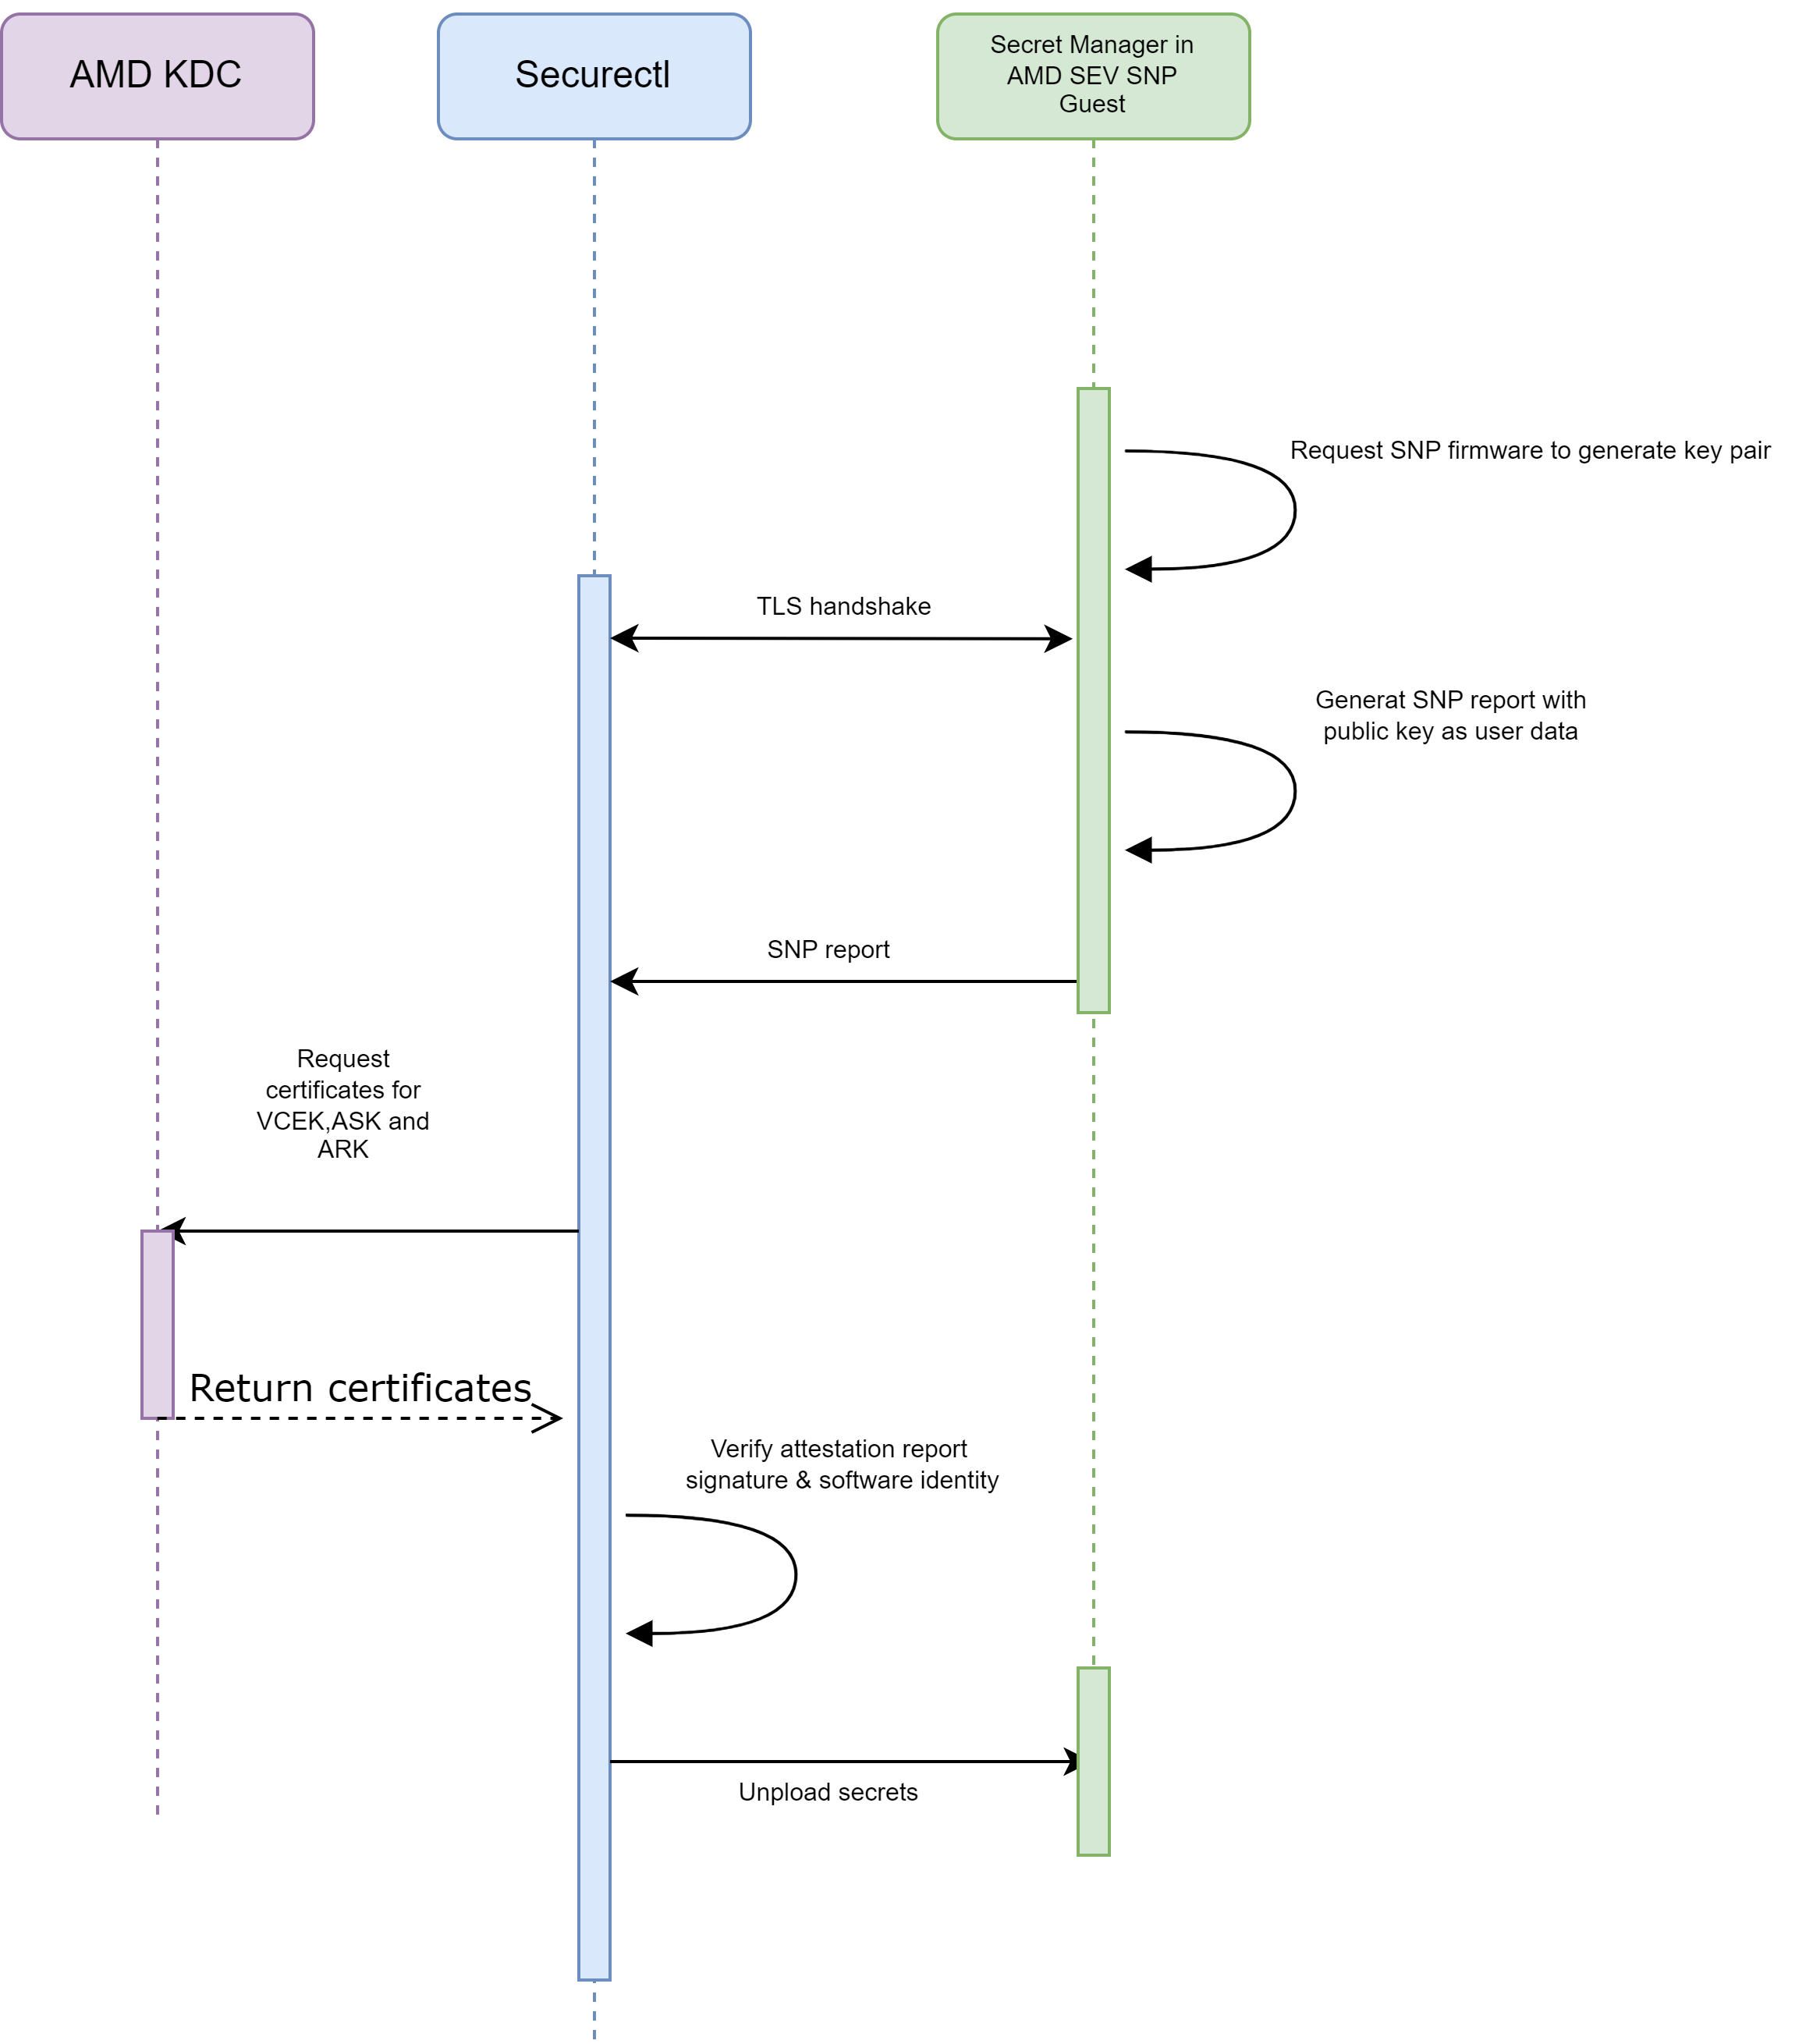
\includegraphics[width=0.8\textwidth]{images/upload_secret.png}
    \caption[Secret Uploading Workflow]{Secret Uploading Workflow. Note that in the figure, the application owner uses Securectl to attest secret manager and upload secrets.}
    \label{fig:upload_secret}
\end{figure}

The process of uploading secrets to the secret manager requires two steps to be taken by the application owner. Firstly, the application owner needs to attest the secret manager. Secondly, a secure channel must be established for the secret uploading.
This process is illustrated in Figure~\ref{fig:upload_secret}. We assume the secret manager is running in the AMD SEV SNP~\cite*{SEV_SNP_white_book}. Initially, 
the secret manager requests SNP to generate a key pair for the TLS connection. The private key of this pair is then stored in the secret manager's memory, which is protected by the TEE.
Since the key pair can only be used by the secret manager, it can be considered as an identifier for the secure channel. To bind the secret manager to the identifier of the secure channel,
the hash of the public key is added to the attestation report of the secret manager. Upon receiving the report, the application owner requests a certificate chain from the AMD KDC using 
the CHIP\_ID and TSB parameters in the report~\cite*{snp_kdc}. The certificate chain is then used by the application owner to verify the signature of the report. Then using the information in the report,
the application owner can ensure that the remote secret manager is genuine and that the hash of the public key used to establish the TLS matches the hash of the public key in the report. 
By fulfilling these steps, the application owner can determines that the entity on the other side of the secure channel is the intended secret manager. Thus, the channel can 
safely be leveraged for the secrets uploading.

\subsection{Secure Application Deployment}

The objective of secure application deployment is to ensure the confidentiality and integrity of an application's sensitive data and the shielding layer's policy. To achieve this goal, a new deployment mechanism is proposed to offload secrets 
management and deployment from Kubernetes, as illustrated in Figure~\ref{fig:attestation_provisioning}.

The cluster operator still uses YAML to deploy applications but without including any secrets. Instead, the application secrets and the policy of the shielding layer are uploaded to the secret manager. The cluster operator only needs to provide the 
IP address of the secret manager and secrets'URL in the YAML. This IP address is used by the remote attestation and provisioning agent to establish a connection with the secret manager during the application process creation, while the URLs are 
employed by the agent to request secrets via the HTTP GET method.

\begin{figure}[H]
    \centering
    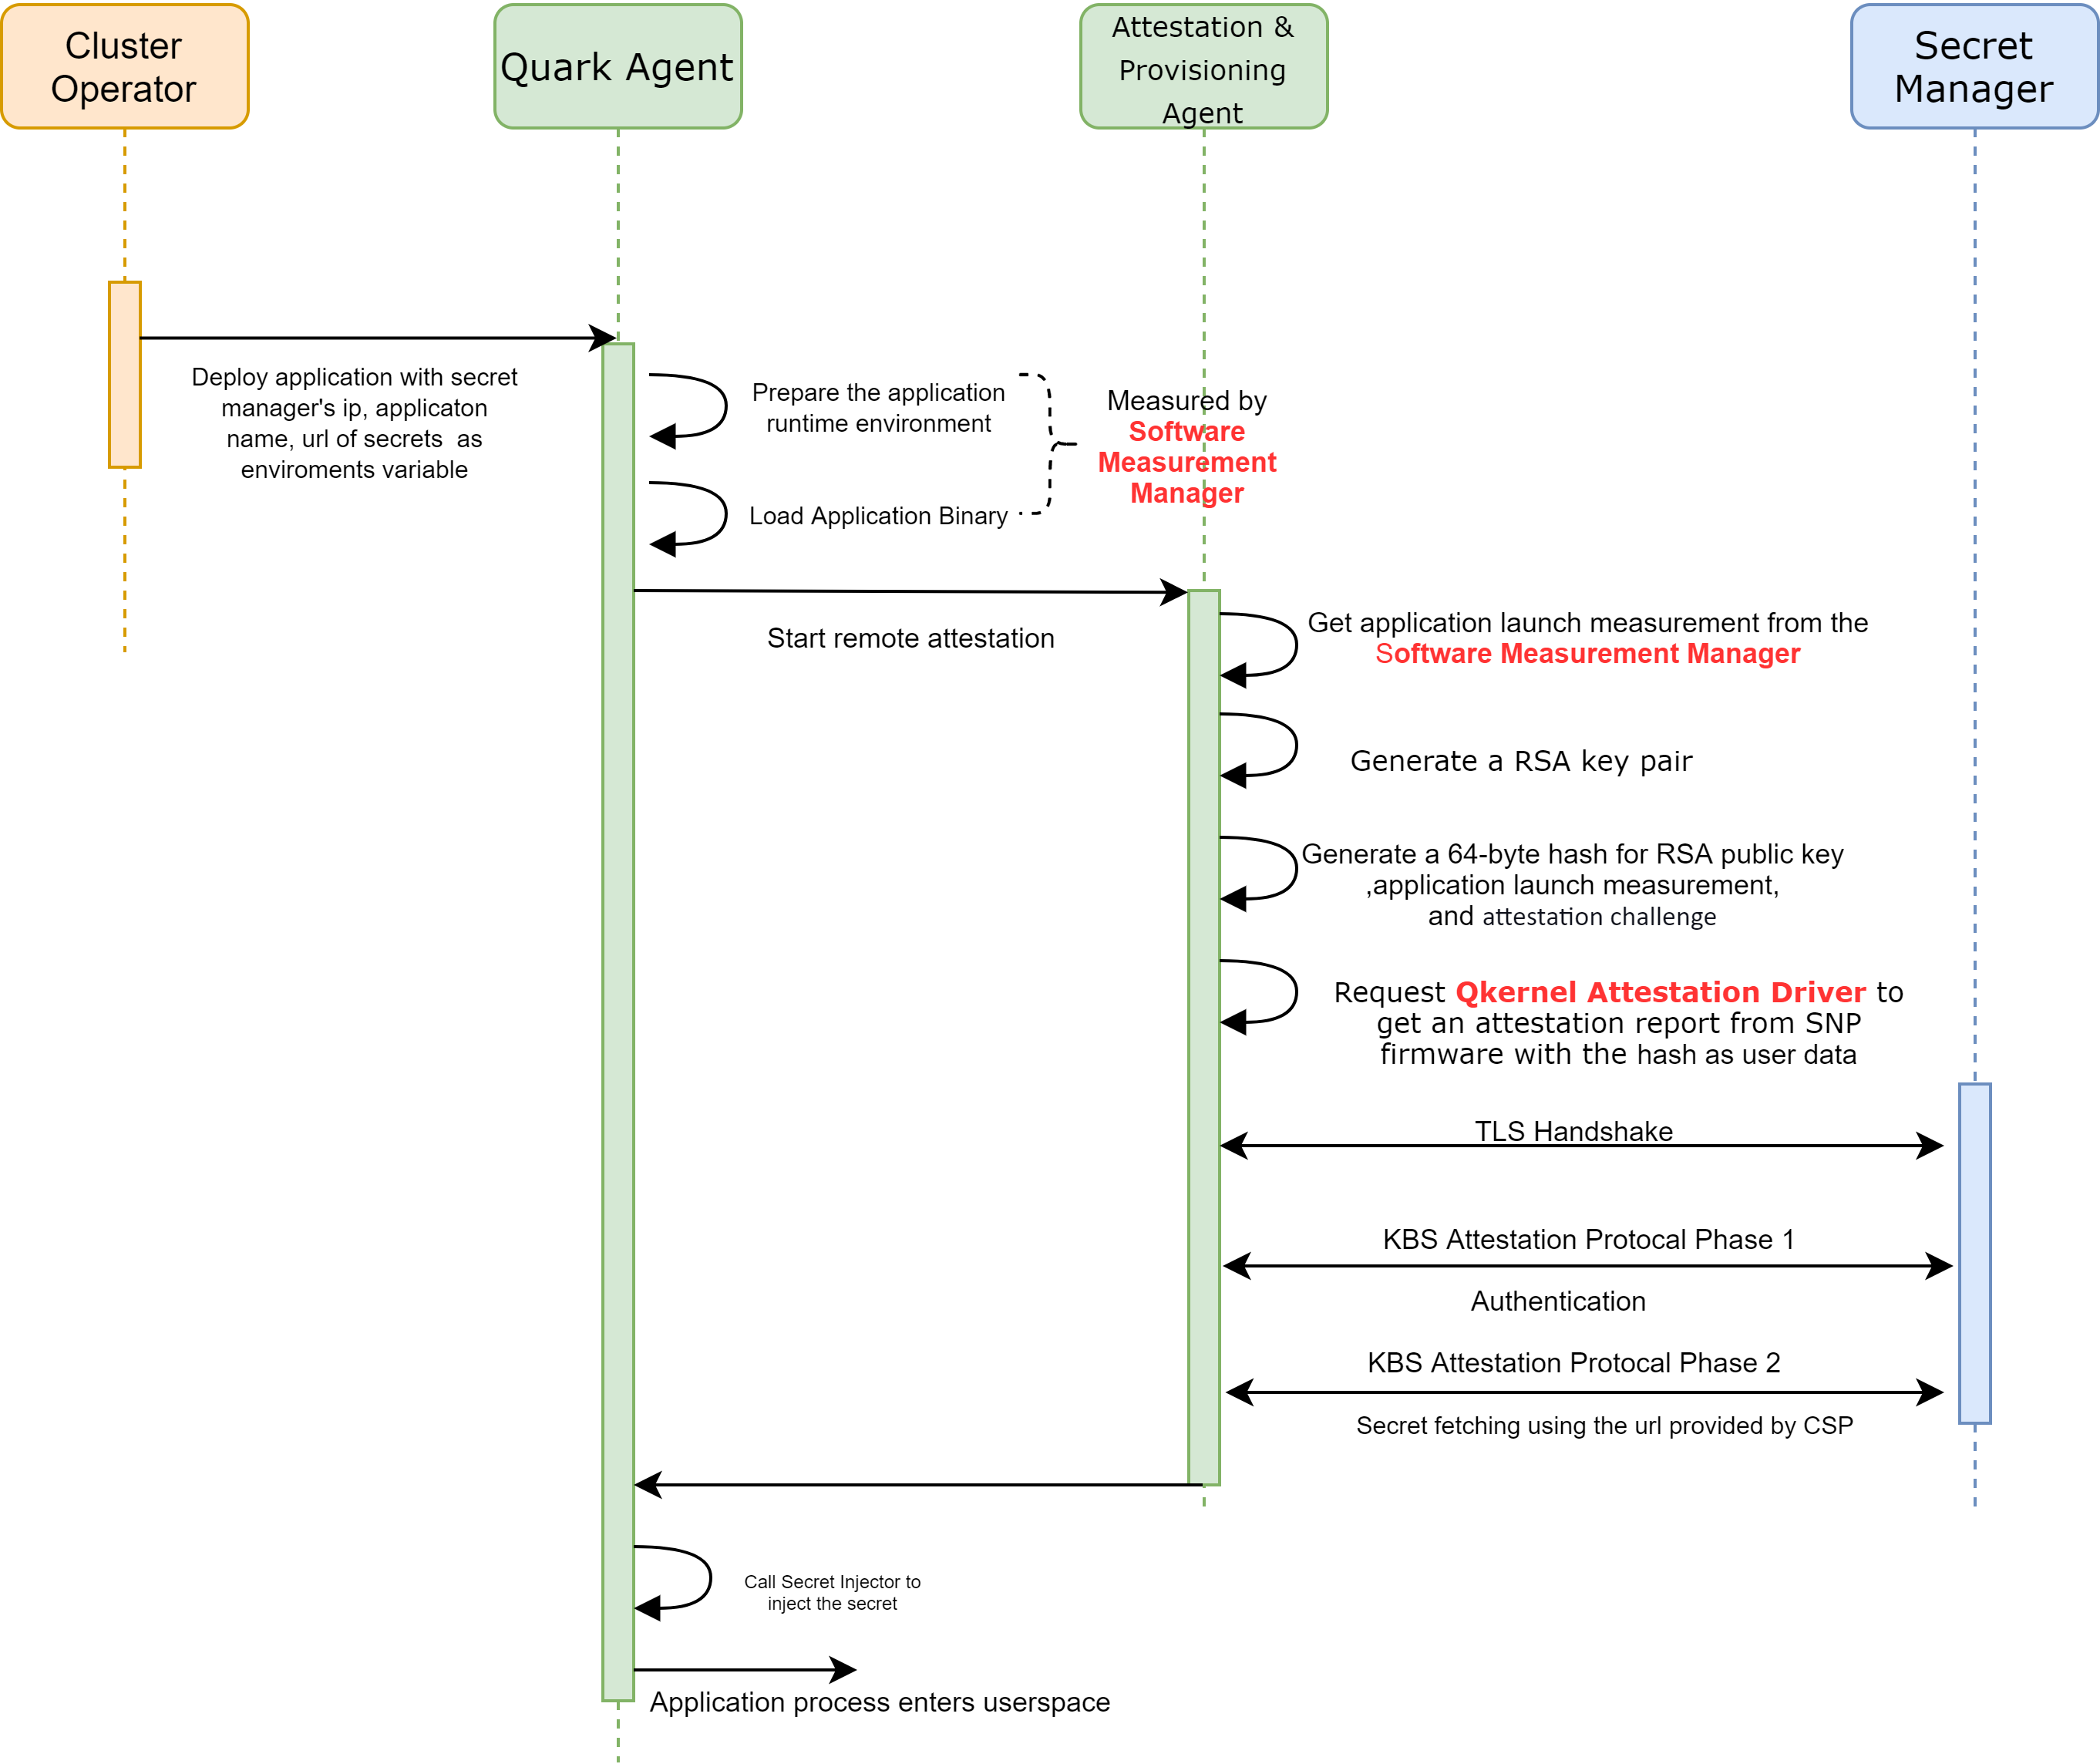
\includegraphics[width=0.8\textwidth]{images/attestation_provisioning.png}
    \caption[Secure Application Deployment Workflow]{Secure Application Deployment. The green components are running in the enclave. The cluster operator is not trusted. The Secret Manager is responsible for managing the secrets as a relying party, attesting  enclave, and provisioning the secrets.}
    \label{fig:attestation_provisioning}
\end{figure}

Upon receiving an application creation request, the quark agent located in the enclave creates the application process based on a process specification. This involves loading the application binaries from the host machine, setting up the file 
system for the application process, etc. To ensure the integrity of the loaded binaries, the software measurement manager extends the loaded binaries with a hash called the enclave start measurement, through which the loaded binaries are bound to 
the enclave start hash. Note that this measurement is constructed at the enclave start, which also includes a measurement of the Qkernel command-line arguments.

\begin{figure}[H]
    \centering
    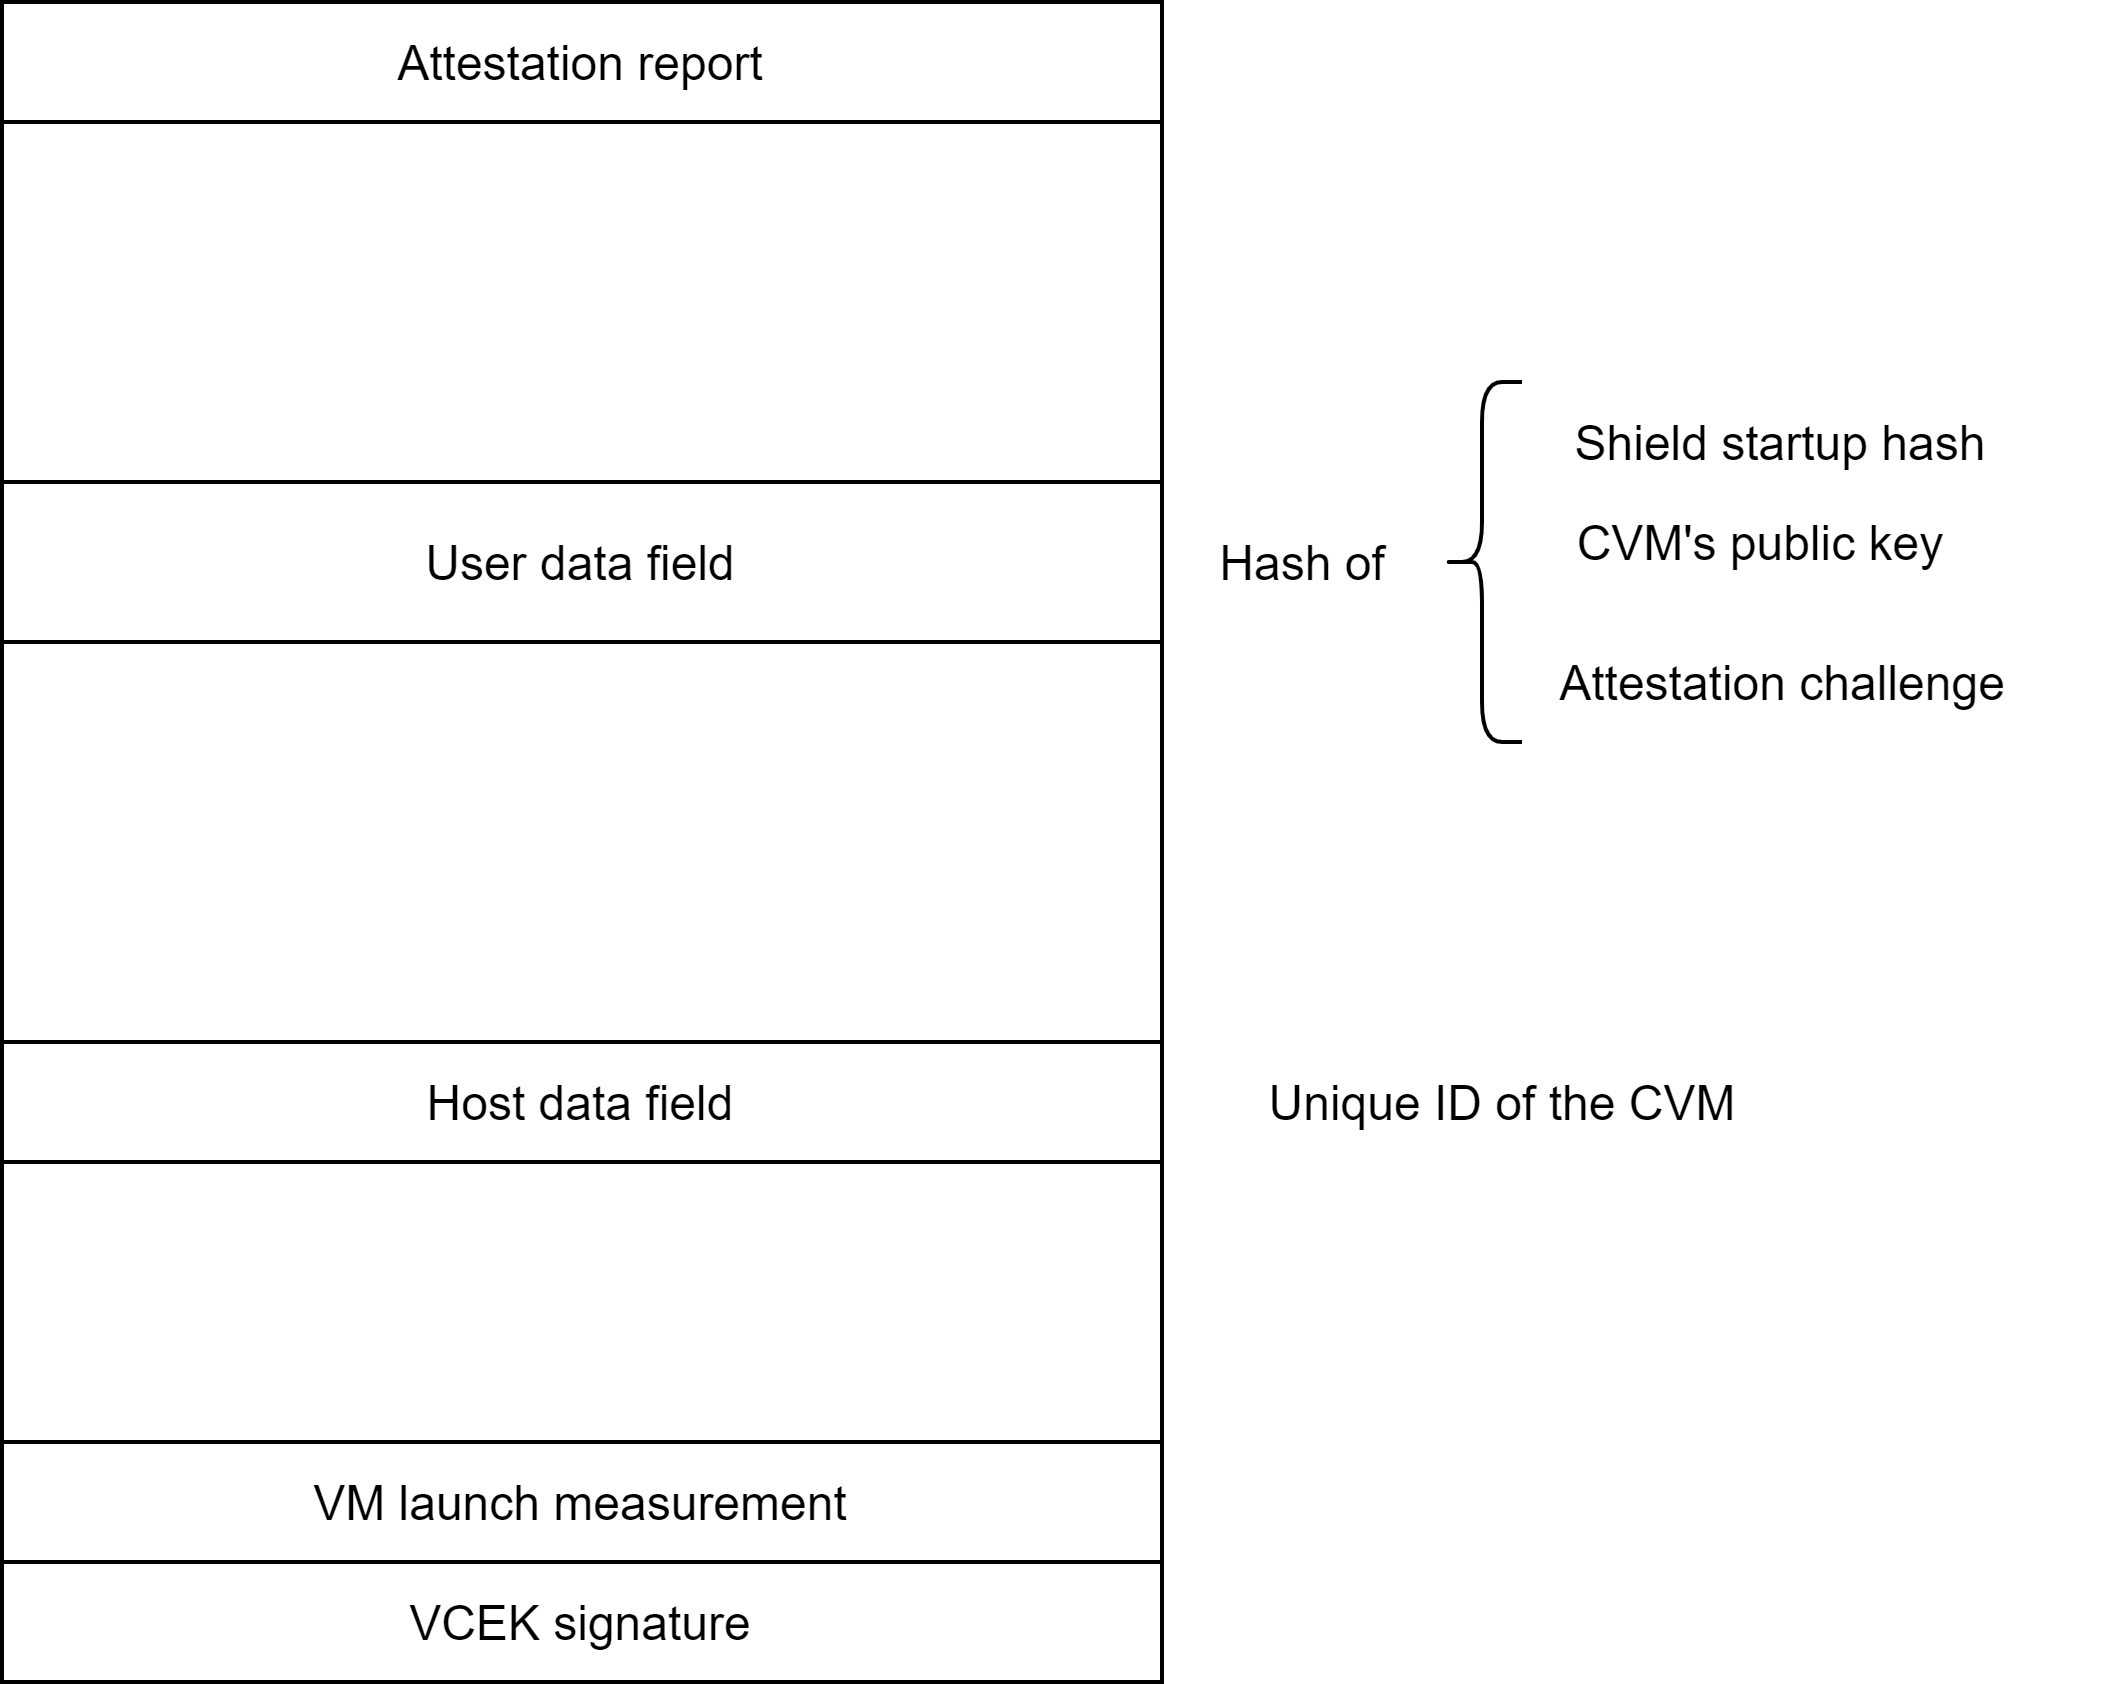
\includegraphics[width=0.8\textwidth]{images/attestation_report_format.png}
    \caption[SNP attestation report]{SNP attestation report.}
    \label{fig:attestation_report_format}
\end{figure}

Subsequently, the remote attestation and provisioning agent requests the Qkernel attestation driver to generate an attestation report. Depending on the type of TEE, the driver will generate a different attestation report. Assuming the enclave runs 
in AMD SNP, the driver will request the SNP firmware to generate the attestation report. Then, the attestation and provisioning agent will connect to the secret manager using the IP address in the YAML and use this report to prove the enclave's 
identity and get secrets from the secret manager following the KBS attestation protocol. The attestation report is shown in Figure 6. It is protected with the VCEK signature and contains:
\begin{itemize}
    \item SNP firmware's measurements for the VM boot process
    \item Tamper-resistant 64-byte user-defined data.
    \item Host data.
    \item VCEK signature.
    \item Others
\end{itemize}


The secret manager verifies the report's signature using the certificate chain required fro AMD KDC~\cite*{snp_kdc}. By examining the virtual machine boot process measurements, the secret manager can confirm that the enclave is using the correct Qkernel binary. 
Since Qkernel is loaded into the enclave memory using SNP\_LAUNCH\_UPDATE~\cite*{snp_firmware} during virtual boot by Qvisor, snp firmware also measures the Qkernel binary. Notably, the code of the shielding layer is part of the Qkernel binary.

The user-defined data in the attestation report is a hash, including the enclave startup measurement and a hash of the TEE-generated public key. The enclave startup measurement is created by the software manager and incorporates all the sensitive 
data that the enclave loads from the host after the enclave starts until the application is loaded. This includes the Qkernel command line parameters, the binaries loaded during the application startup, and the secret manager's public key. By 
comparing the enclave startup measurement with the reference hash provided by the application owner, the secret manager can verify that the enclave is appropriately configured and that only legitimate binaries are loaded.

To establish a secure channel for secrets provisioning, the KBS attestation protocol~\cite*{kbs_Attestation_protocol} necessitates that the enclave generates an asymmetric key pair from TEE. During the authentication phase of the protocol, the public key is sent to the secret 
manager with an attestation report. In the second phase, the secret manager uses this public key to encrypt the secret requested by the enclave. By incorporating the public key hash in the enclave's attestation report, the secret manager can 
determine that the public key belongs to the enclave, and only the enclave can decrypt the encrypted secret.

To prevent an attacker from hijacking the secret manager's address and impersonating the secret manager, the remote attestation and provisioning agent use the secret manager's public key to verify the secret manager's identity during the TLS 
handshake. Note that Kubernetes mount the public key of the secret manager as a file on the application's rootfs. To this end, an attacker can provide a bogus public key to the remote attestation and provisioning agent to trick it into establishing 
a connection with the fake secret manager. To address this, the remote attestation and provisioning agent reads the secret manager's public key into the guest's memory and add the key's measurements to the enclave startup measurement. This way, 
the secret manager can verify that the remote attestation and provisioning agent uses the correct public key. When an attacker presents the remote attestation and provisioning agent with a fake secret manager's public key, the TLS handshake fails 
due to a mismatch between the public key and the certificate of the real secret manager. Even if the TLS is established, the real secret manager will reject the authentication request from the agent because the enclave startup measurement does not 
match the reference hash.

Since all enclaves use a standard Qkernel binary and applications are created from standard images, the attestation evidence cannot uniquely identify an enclave. Instead, the evidence only certifies that the attester is an enclave running in a 
TEE with the correctly loaded application. Hence, If the secret manager identifies the enclave only based on the attestation evidence, an enclave belonging to one stakeholder could steal the secrets of another stakeholder. To circumvent this, 
the application owner should assign a unique ID to each enclave. This ID should be added to the host data field in the attestation report by Qvisor during enclave setup using SNP\_LAUNCH\_FINISH~\cite*{snp_firmware}. This field is immutable after launching the enclave, 
so the ID is bound to the enclave's attestation evidence. When the secret manager receives an enclave's attestation report, it can use this ID to determine its identity. In the authentication phase of the KBS attestation protocol, the secret 
manager assigns a cookie identifier to an enclave's HTTP request, binding the enclave's ID and attestation result to the cookie identifier. In the second phase, the secret manager maps the cookie identifier in the attester's resource request message 
to its attestation result and the enclave's ID. The secret manager uses this information and the data owner-defined policy to determine whether to grant access to a particular secret to the attester. 

The attester's resource request URL has the following format: <repository>/<type>/<tag>, where <repository> is similar to the concept of container image repository, <type> is used to distinguish between different resource types, and <tag> is used 
to distinguish between different versions of a resource. In the secret manager, each user has a unique repository. The secret manager allows users to specify which enclaves with which IDs can access this repository. In this way, we effectively avoid 
cross-leakage of secrets between different stakeholders.

\subsection{Application Runtime Attestation Service}
\label{sec:runtime_attesation}

An application may need to authenticate itself to a remote end at runtime. Quark attestation and provisioning infrastructure enable applications to obtain attestation reports through the guest system call interface. 
Depending on the application's needs, one of three report formats can be obtained: an attestation report generated by the TEE hardware and two software attestation reports created by the shielding layer. The latter contains:
\begin{itemize}
    \item Enclave start-up measurement.
    \item Enclave ID.
    \item Signature.
    \item Sixty-four bytes of application-specified data.
  \end{itemize}

The application can choose to sign the software report with a key issued by the secret manager or by a key it provided. The secret manager key is sent to the enclave along with the application's secret during the creation of the application process. 
Software reports offer additional possibilities for how the application proves its identity to the remote end. In other words, the remote end can verify the report without the assistance of the hardware provider. Upon verification of the report, 
the remote end can ensure that the application is as expected by using the enclave start-up measurement. Additionally, application-defined data in a software report is tamper-proof, similar to user data in SNP reports. As previously discussed, the 
enclave ID guarantees that the remote end can determine the application's identity, which prevents secret cross-leakage.



\section{Enclave Runtime Measurement}
\label{sec:Enclave_Runtime_Measurement}
Enclave runtime measurements are crucial due to the security analysis findings discussed in Chapter~\ref{sec:security_analyse}. Qkernel command line parameters, the application binary, and shared libraries are loaded from the host. Thus, an attacker can modify them 
to breach the enclave's confidentiality. However, AMD SEV SVP does not facilitate enclave runtime measurements~\cite*{snp_firmware}, and INTEL TDX only allocates four registers for this purpose~\cite*{Intel_tdx_whitepaper}. Consequently, we provide a software measurement manager in the shielding 
layer to measure the data loaded from the host while the enclave is running. The software measurement manager obtains the following important measurements by measuring these data.

\textbf{Enclave startup measurement.} This value refers to the measures of host-loaded data from the enclave starting until the enclave finishes loading the application binaries. To config the application's execution environment, the enclave may have to 
execute multiple binaries first. For example, Nginx startup necessitates the enclave to execute a docker-entry.sh shell script\cite*{nginx}. The shell script then executes several Linux commands. Each is a binary. Therefore, the enclave startup measurement may 
comprise binaries, shared libraries, Qkernel boot parameters, and the secret manager's public key. The attestation and provisioning agent include this measurement in the attestation report, which is conveyed to the secret manager. The secret manager 
compares the measurement to the reference value provided by the enclave owner to ensure that the enclave is genuine.

\textbf{Application startup measurement.} This value records the measure of all binaries and shared libraries loaded from the time the enclave receives the application creation request to the point when the enclave completes loading the application binaries. 
This measurement is a subset of the enclave startup measurement and is stored in the enclave memory. It serves as a reference hash with the application restart measurement.

\textbf{Measurement of binaries at application runtime.} The application process loads its shared libraries after it enters the user space. Moreover, the enclave creates a process and loads the corresponding binary from the host when a user initiates a 
command to the application. The software measurement manager measures the loaded binaries or shared libraries to prevent an attacker from serving compromised binary to the enclave. However, unlike the enclave startup measurement, which is forwarded 
to the secret manager, the runtime measurements are verified by the software manager. The shielding layer's policy holds reference measurements for the runtime binaries, as shown in Figure~\ref{fig:measurement}. In this case, the software measurement manager measures 
the binaries and compares the result with reference values from the policy. If the two values differ, the enclave will panic. This ensures that during application runtime, the correct binaries are loaded.

\begin{figure}[H]
    \centering
    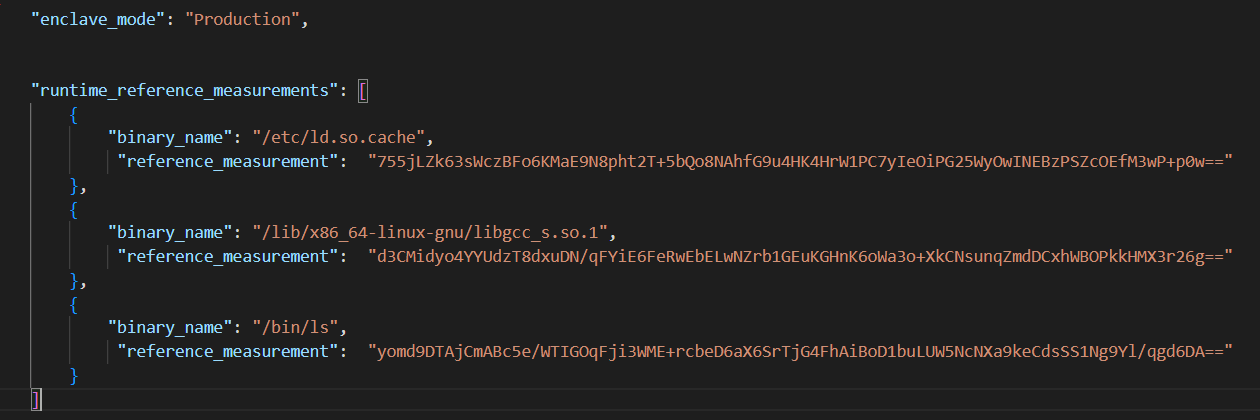
\includegraphics[width=0.8\textwidth]{images/measurement.png}
    \caption[Reference Value in Shielding Layer's Policy for Runtime Binary Measurement]{Reference Value in Shielding Layer's Policy for Runtime Binary Measurement}
    \label{fig:measurement}
\end{figure}

\textbf{The application restart measurement.} In the event of an application crash where the enclave is not exited, Kubernetes will attempt to restart the application within the enclave. The enclave will therefore recreate the application process, load the relevant 
binaries, and inject secrets stored in the enclave's memory. An attacker may exploit this situation by injecting malicious code into the enclave to retrieve secrets, thereby breaching the enclave's confidentiality. One potential solution is to 
measure the loaded binaries or shared libraries during the application restart and send the result to the secret manager for verification. However, this approach is costly as it involves generating an attestation report and communicating with the 
secret manager via the network. Therefore, the software measurement manager stores application startup measurement and uses it as a reference hash for application restart measurement. If the two do not match, the enclave will panic. In doing so, 
the enclave ensures that the binary loaded at restart is identical to the binary loaded during the initial application launch. As the binary's measurements during the first launch are sent to the secret manager for integrity checking, comparing the 
two hashes guarantees the integrity of the loaded binary during application restart.

Regarding obtaining the reference values for enclave startup measurement and measurement of individual binaries loaded at application runtime, we implemented a developer mode for the enclave. When running in developer mode, the enclave prints the 
enclave and application runtime measurements for each binary and shared library to the Qkernel log on the host. The application owner should operate the enclave in a trusted environment to obtain these reference values.


\section{New Pattern for EXEC Requests}
\label{sec:design_EXEC_Requests}
\subsection{Overview}



\begin{figure}[H]
    \centering
    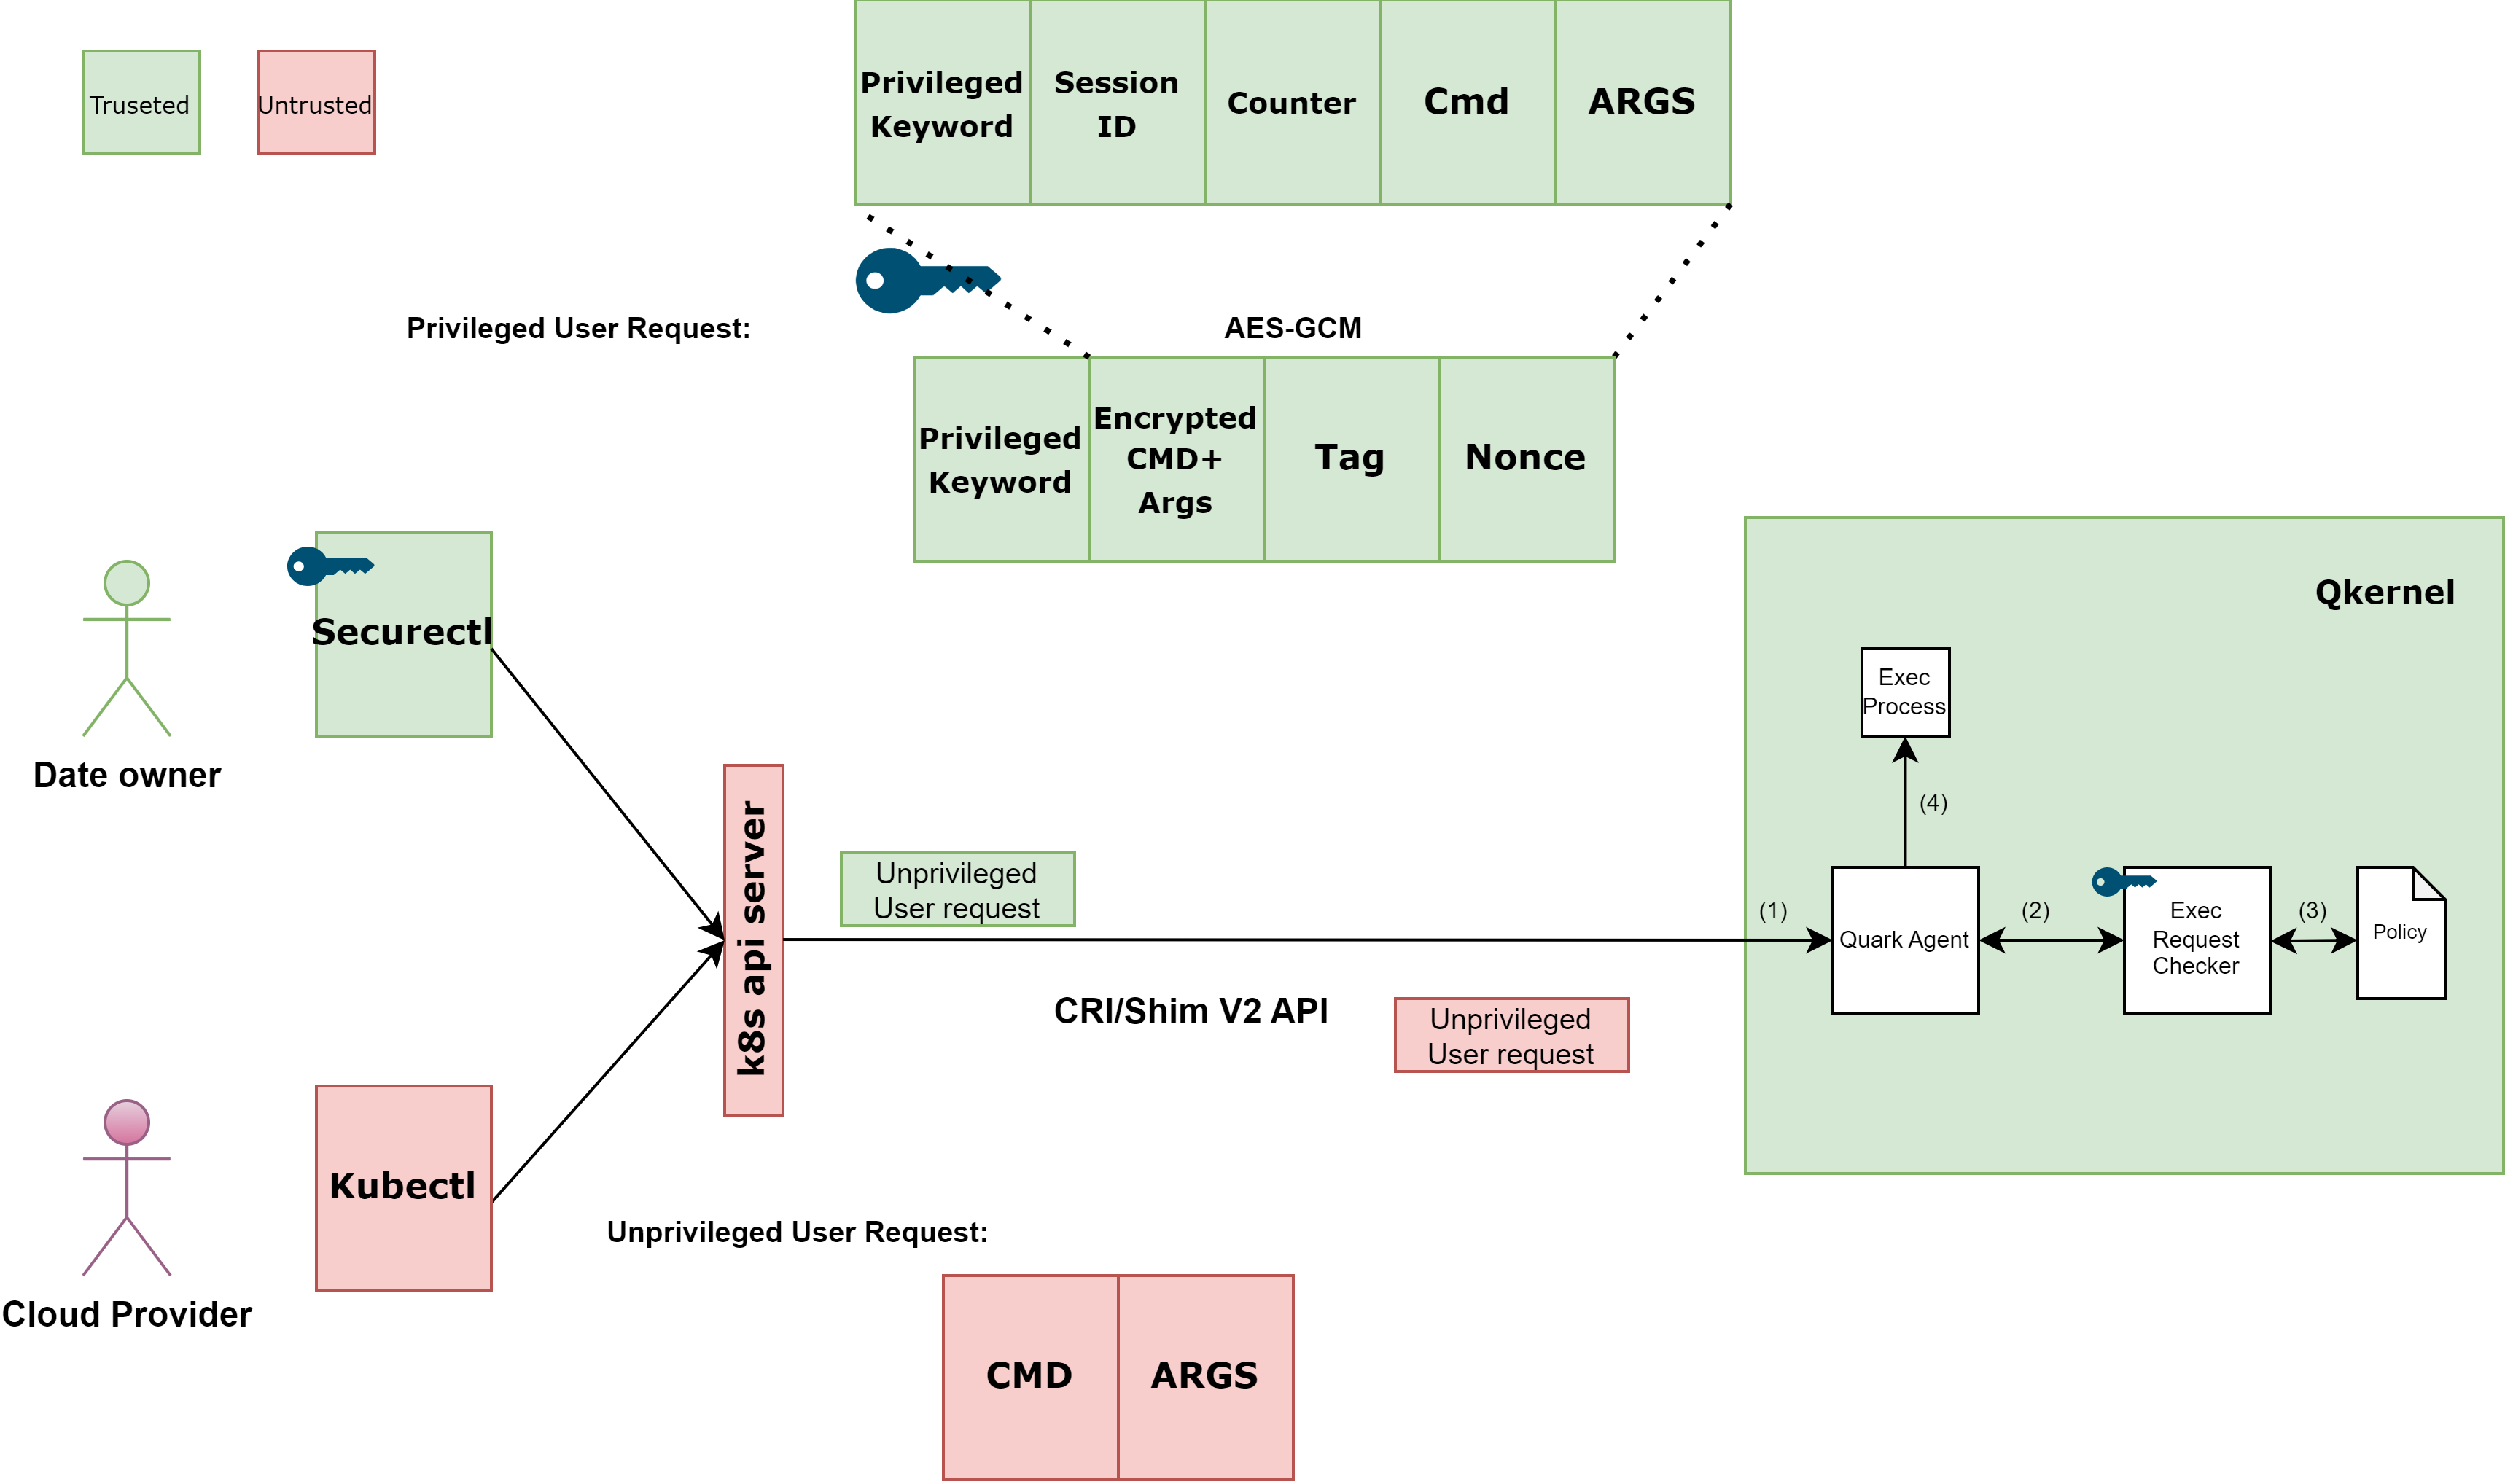
\includegraphics[width=0.8\textwidth]{images/new_pattern_of_exec.png}
    \caption[New Pattern for EXEC Requests]{New Pattern for EXEC Requests}
    \label{fig:new_pattern_of_exec}
\end{figure}


Any user can send an EXEC request to an application. As analyzed in Chapter~\ref{sec:security_analyse}, when a user issues a command to an application or allocates a terminal, Kubernetes will send an EXEC request to the Quark agent located in the enclave. After receiving 
the request, the Quark agent creates a process to execute the command binary (For a terminal allocation request, the command is /bin/bash). Note that the o only difference between issuing a command and allocating a terminal is that the terminal 
keyword is true in the process specification of the exec request for allocating a terminal. Thus, we refer to both issuing a command and allocating a terminal collectively as the EXEC request. Since the Quark agent lacks authentication and access 
control for EXEC requests, an attacker can send arbitrary EXEC requests to an application. Therefore, a new pattern for EXEC requests is proposed, illustrated in Figure~\ref{fig:new_pattern_of_exec}.

The pattern divides EXEC requests into two categories, namely privileged and unprivileged EXEC requests. Privileged EXEC requests are issued by privileged users, i.e., the application owner, while non-privileged requests are issued by untrusted 
entities. An untrusted entity here refers to someone other than the application owner. Privileged and unprivileged users send privileged or unprivileged requests to the enclave using secretctl or kubectl, respectively. Both requests are redirected 
to the enclave through the Kubernetes  API server and the CRI, Shim V2 API interface. Upon receiving the EXEC request, the Quark agent forwards it to the Exec request checker. The Exec request checker will authenticate and access control the request 
according to the enclave policy, as shown in Figure~\ref{fig:exec_policy}. The Quark agent will decide whether to create the EXEC process based on the results returned by the Exec request checker.
\begin{figure}[H]
    \centering
    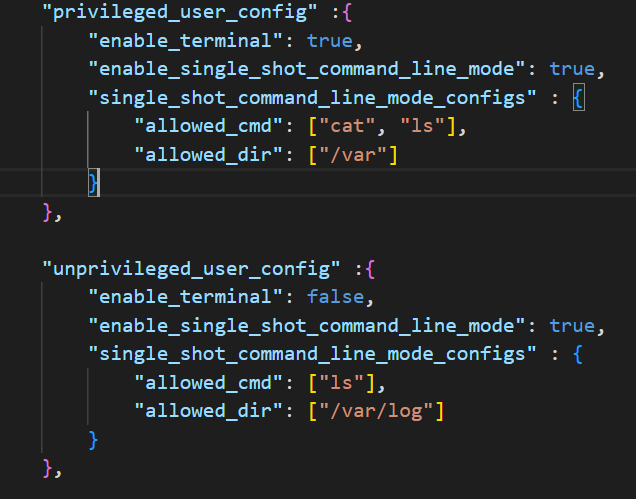
\includegraphics[width=0.8\textwidth]{images/exec_policy.png}
    \caption[Policy for EXEC Requests]{Policy for EXEC Requests. This EXEC request policy is part of the enclave policy. The enable\_teminal keyword specifies whether a terminal can be 
    allocated. For example, kubectl exec -it command will be rejected when enable\_teminal is set to false for unprivileged users. The keyword enable\_single\_shot\_command\_line\_mode 
    defines whether users are allowed to issue a command. When this keyword is false in the non-privileged user's configuration, any commands issued by a user using kubectl will be 
    rejected. When this keyword is true, the application owner must restrict which commands are allowed and which directories the commands have access to. This is done through single\_shot\_command\_line\_mode\_configs in the enclave policy.}
    \label{fig:exec_policy}
\end{figure}



\subsection{Protection for Privileged Exec Request}
Since privileged EXEC requests are transmitted through the Kubernetes  component to the enclave, the authenticity, integrity, and confidentiality of the commands and their parameters in requests must be protected. In addition, we must implement a mechanism 
to distinguish between privileged and unprivileged requests. This can be achieved through the frame structure as in Figure~\ref{fig:new_pattern_of_exec} and the use of authenticated encryption operations with associated data, i.e., the Advanced 
Encryption Standard Galois/Counter Mode (AES-GCM)~\cite*{aes_gcm}. The frame structure encapsulates the AES-GCM's random number (nonce) for secret decryption, the authentication Tag, the encrypted payload, and the keyword 'Privileged'. Since the Open Container 
Initiative requires that commands and their arguments be passed as a vector of strings, the encrypted payload, nonce, and tag are encoded in base64. The plaintext payload contains the keyword 'Privileged,' the session ID, a counter, the command, 
and its parameters.

AES-GCM~\cite*{aes_gcm} ensures the confidentiality, authenticity, and integrity of privileged EXEC requests. Besides, it is easy to deploy as it requires only a shared key. After a successful remote attestation, a key is shared between the application owner and 
the enclave. The application owner can use this key to encrypt privileged commands and their parameters. When the enclave receives a privileged request, the exec request checker can use the key to confirm that the request was generated by a 
privileged user who knows the key (authentication), verify the request's integrity, and decrypt the request.


The keyword "Privileged" is used to distinguish privileged from non-privileged commands. The Kubernetes API requires the user to pass a command, and it's parameters as an array of strings, where the first element is the command and the remaining elements 
are the parameters, e.g. ["cat", "/var/log"]~\cite*{k8s}. Privileged-level commands are passed to the enclave as string arrays through the Kubernetes  API, just like non-privileged-level commands. Thus, the string arrays corresponding to privileged-level commands have 
the following format ["Privileged", "Encrypted cmd + arg," "Tag ","Nonce"]. When the exec request checker receives an EXEC request, it can determine if it is privileged by checking the first element of the command array. Note that the command array 
is part of the EXEC request process specification known as args.


The  monotonic counter and session are designed to prevent reply attacks. Since the privileged Exec requests are transmitted to the enclave by Kubernetes , an attacker can intercept a privileged request and send it continuously to the enclave to 
interfere with its operation. In addition, it can analyze the execution result of an EXEC request. Although the result is encrypted, it may get different results from executing the same command twice. In this case, it may be possible to derive the 
plaintext by analyzing the changes in the ciphertext.   Therefore, we introduce a monotonic counter for privileged-level EXEC requests. This counter is assigned by the enclave to privileged users. When the value of the monotonic counter in an EXEC 
request is smaller than the reference value stored in the enclave, the request is rejected. Since there may be more than one privileged user, it is not easy to share the counter. Therefore, we introduce sessions. In this case, the enclave will 
assign each privileged user a random session id and a unique counter. This id and counter are stored in the enclave and will be sent to a privileged user via a secure channel. The privileged user can use the session id and counter to construct a 
privileged EXEC request. Note that the counter is added by one after each EXEC request.


With the session and counter, we avoid the following two reply attacks. First, the attacker sends a request that belongs to an illegal session, i.e., the session id is not stored by the enclave. Second, the attacker has sent an outdated request to 
the enclave. This means that the counter value in a request is less than the current counter value recorded in the enclave for the requested session ID. In this case, the enclave will refuse to execute it.

\subsection{Session Assignment}

Figure~\ref{fig:session_base_auth} demonstrates how a privileged user gets a session. In the login phase, a privileged user submits a login request using securectl. The login request is a privilege EXEC. However, the payload of the privileged EXEC 
request contains the keyword Login plus a random number instead of a real Linux command. The random number is used to prevent reply attacks. When the request is received and verified by the enclave,  it assigns a session id and a unique counter to 
the privileged user. These two values are stored in the enclave and returned to securectl. The enclave returns these two values via the stdout of the exec process.

\begin{figure}[H]
    \centering
    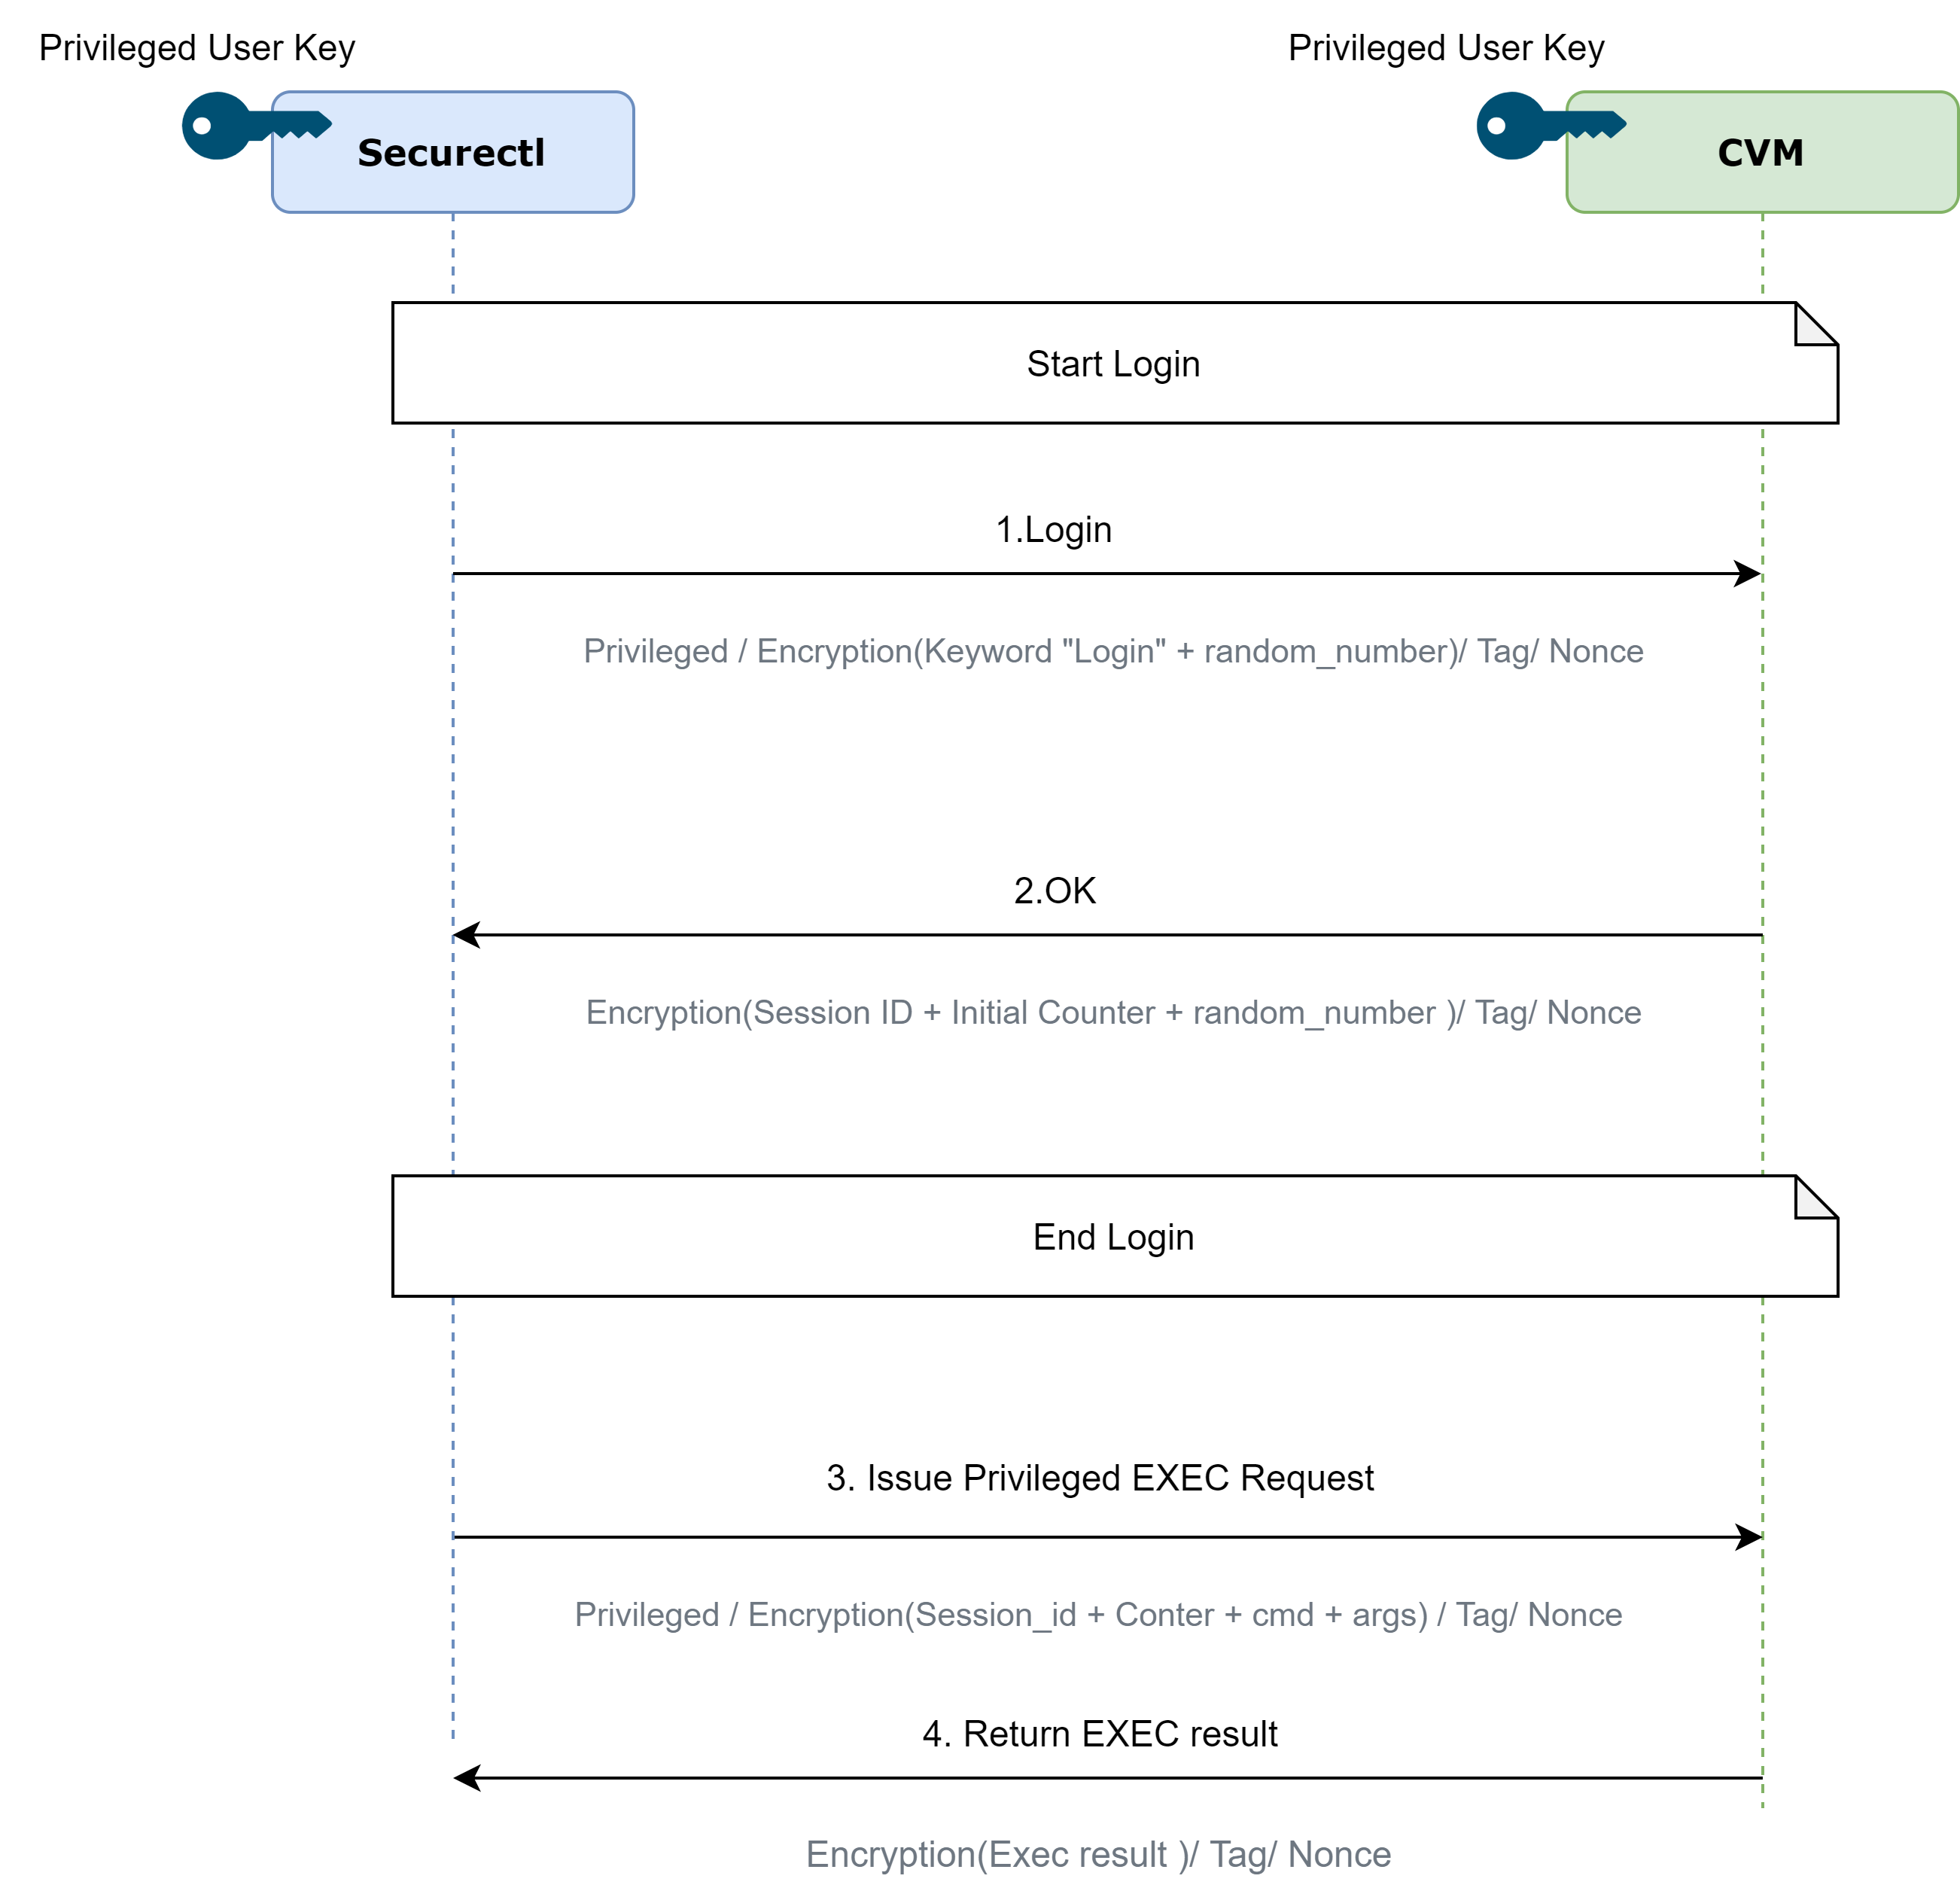
\includegraphics[width=0.8\textwidth]{images/session_base_auth.png}
    \caption[Session Assignment]{Session Assignment}
    \label{fig:session_base_auth}
\end{figure}

When the enclave receives the exec request, it creates a process based on the exec request's process specification. However, the keyword "Login" is not a Linux command. Thus, the enclave replaces the command executed by the exec process with "ls." 
Once the process completes running ls and writes the result to the process's STDOUT, the STDIO shield intercepts the data written to STDOUT and replaces it with the privileged user-assigned session ID and counter. Since the login request is 
privileged, its output is cryptographically protected.


\section{Guest User Space Process STDIO Protection}
\label{sec:design_STDIO_PROTECTION}
The enclave generates guest user-space processes based on process specifications for application creation and EXEC requests. These processes' standard input and output are either tty (Terminal IO) or named pipe (Normal IO), depending on the value of 
the Terminal keyword in the specification. As per our security analysis in Chapter 3, the results of application logs and EXEC requests are returned by the process's standard output or standard error streams. Since the standard output and errors 
are redirected to the containerd, cryptographic protection of the standard output and errors for application processes and privileged EXEC processes is essential.

On the other hand, when STDIO of these processes is of the TERMINAL type, the communication between the user and the processes occurs via the terminal IO redirection thread in quark-shim and the tty driver in the host kernel. This means that any 
commands sent by the privileged user and the command execution results are visible to untrusted entities. Specifically, user commands are transmitted via STDIN to the process, which returns the result to the user via STDOUT or STDERR. Consequently, 
when the STDIO type of the process is TERMINAL, encryption is necessary to protect the stdin.

\subsection{Distinguish the STDIO type of the processes}
Encrypting the STDIO of all processes is not a viable solution for several reasons. Firstly, it would impede non-privileged users from accessing the execution results of non-privileged EXEC requests. In addition, when the enclave is running in 
developer mode, application owners may opt out of encrypting the STDIO of the application as it would use kubectl for viewing application logs or issuing commands. Consequently, we classify the file descriptors used as a guest user process's STDIO 
by the process type:

\begin{itemize} \captionof{enumcnt}{List of file descriptor type used as a guest user process's STDIO}\label{dolist}
    \item Application\_Normal\_IO\_STDIN: the application process's STDIN file descriptor for the normal io 
    \item Application\_Normal\_IO\_STDOUT: the application process's STDOUT file descriptor for the normal io 
    \item Application\_Normal\_IO\_STDERR: the application process's STDERR file descriptor for the normal io 
    \item Application\_Termianl\_IO:  the application process's STDIO file descriptor of tty type 
    \item Privileged\_EXEC\_Process\_With\_Terminal\_IO: privileged EXEC process's STDIO file descriptor of tty type
    \item Unprivileged\_EXEC\_Process\_With\_Terminal\_IO: unprivileged EXEC process's STDIO file descriptor of tty type 
    \item Privileged\_EXEC\_Process\_With\_Normal\_IO\_STDIN: privileged EXEC process's STDIN file descriptor for the normal io 
    \item Privileged\_EXEC\_Process\_With\_Normal\_IO\_STDOUT: privileged EXEC process's STDOUT file descriptor for the normal io.
    \item Privileged\_EXEC\_Process\_With\_Normal\_IO\_STDERR: privileged EXEC process's STDERR file descriptor for the normal io
    \item Unprivileged\_EXEC\_Process\_With\_Normal\_IO\_STDIN: non-privileged EXEC process's STDIN file descriptor in the normal io 
    \item Unprivileged\_EXEC\_Process\_With\_Normal\_IO\_STDOUT. non-privileged EXEC process's STDOUT file descriptor for the normal io
    \item Unprivileged\_EXEC\_Process\_With\_Normal\_IO\_STDERR: non-privileged EXEC process's the stderr file descriptor for the normal io.
    \item Login\_EXEC\_Process\_STDIN: STDIN belonging to the Login exec process
    \item Login\_EXEC\_Process\_STDERR: STDOUT of the Login exec process
    \item Login\_EXEC\_Process\_STDOUT: STDERR of the Login exec process
    
\end{itemize}

In cases where the STDIO type of the application process is terminal, a tty slave will be used for STDIN, STDOUT, and STDERR. The type of this tty slave is Application\_Termianl\_IO.  In contrast, if it is Normal\_IO (named pipe), then the STDIN, 
STDOUT, and STDERR will correspond to Application\_Normal\_IO\_STDIN, Application\_Normal\_IO\_STDOUT, and Application\_Normal\_IO\_STDERR, respectively. The unprivileged EXEC process's STDIO is not encrypted by default. For standard streams of 
application and privileged EXEC processes, the enclave allows the application owner to specify a policy to decide whether they should be cryptographically protected.
\begin{figure}[H]
    \centering
    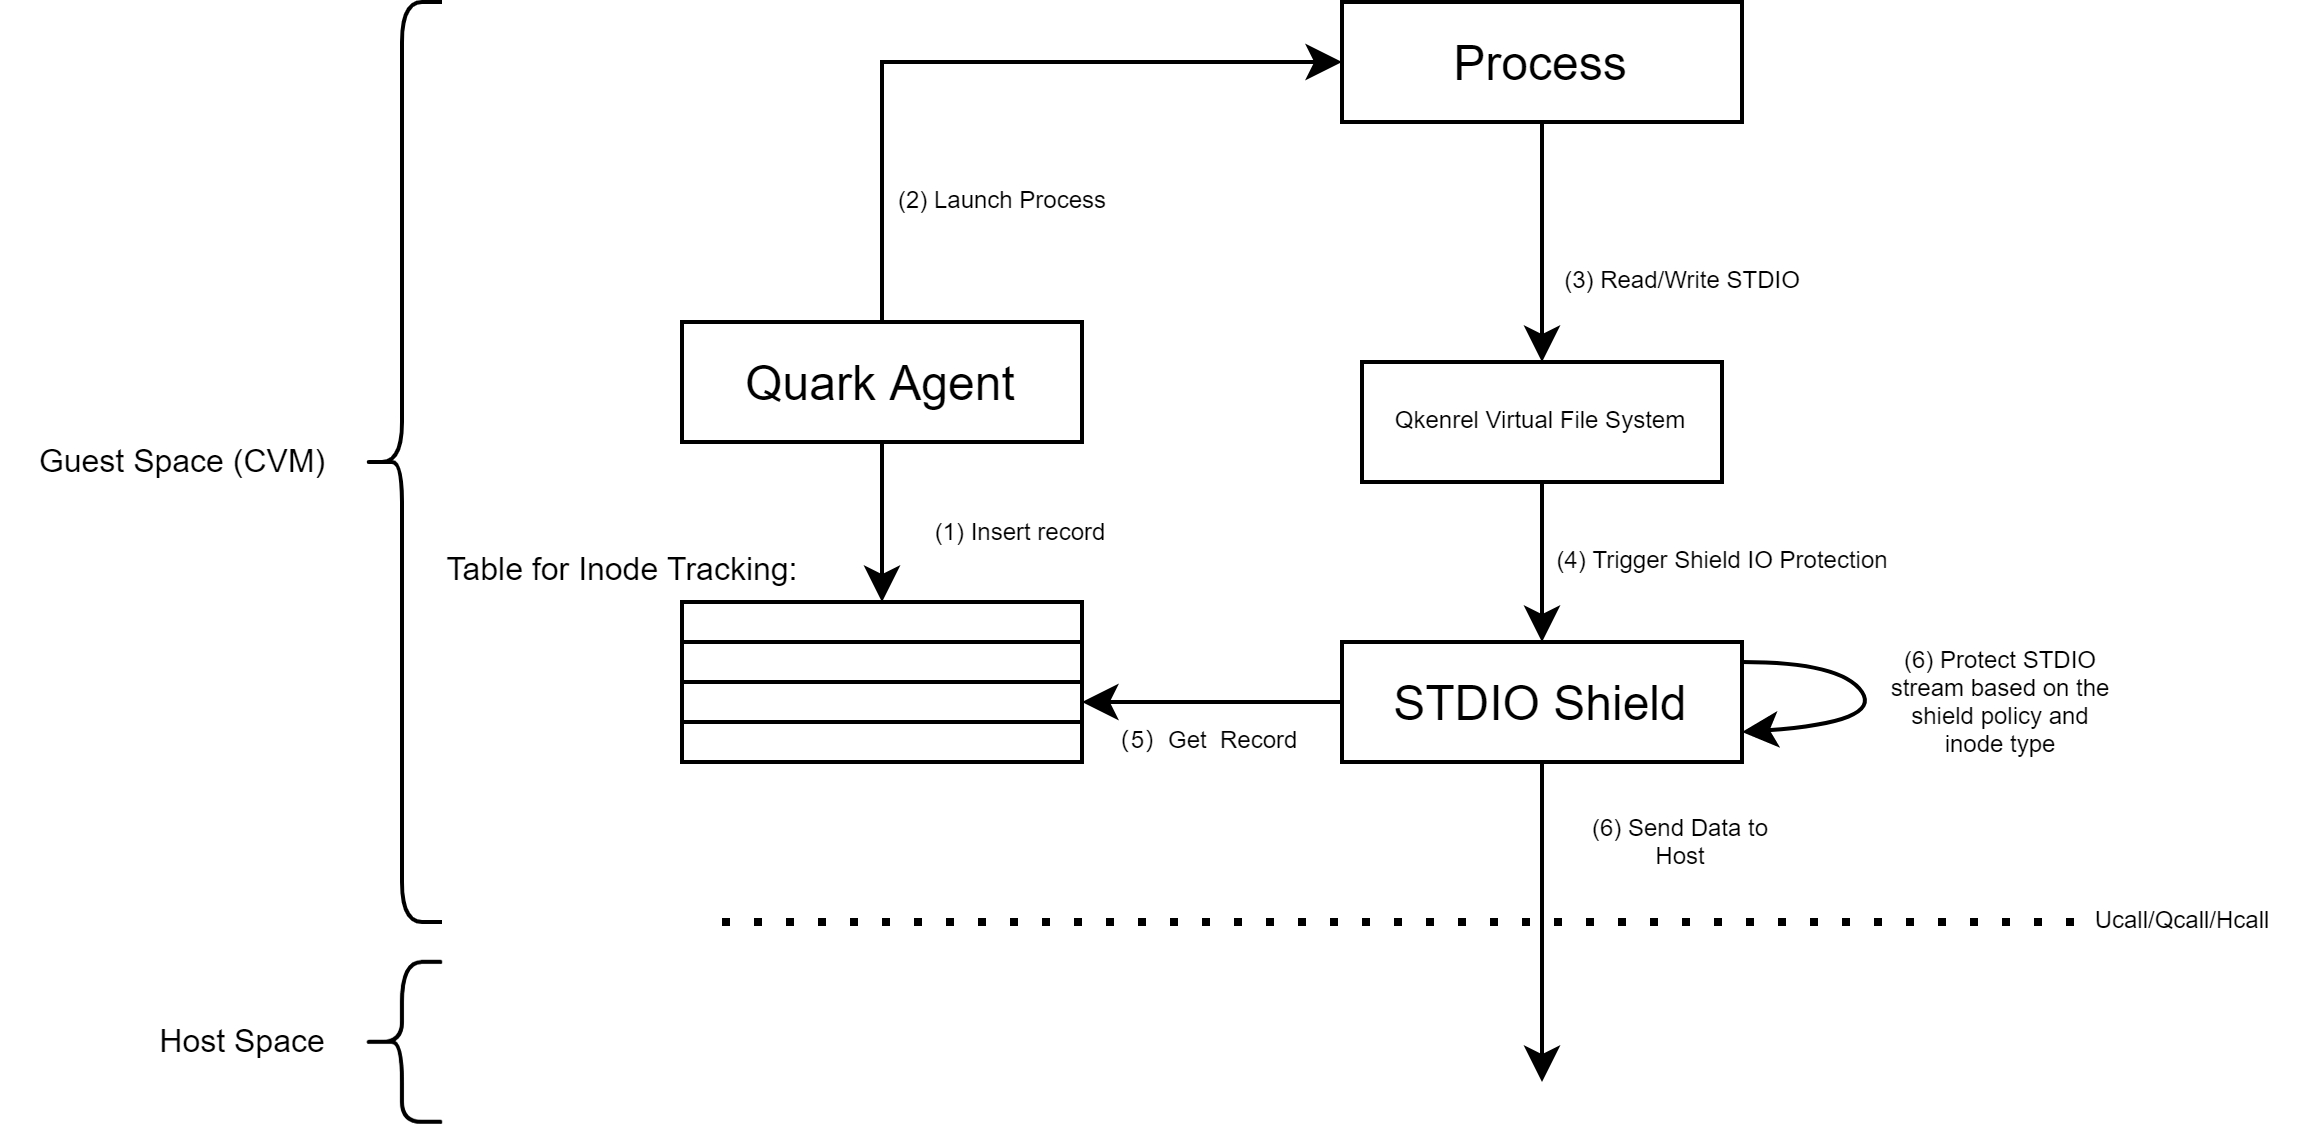
\includegraphics[scale=0.5]{images/differenciate_fds.png}
    \caption[Distinguish file descriptor type used as guest user processes' STDIO]{Distinguish file descriptor type used as guest user processes' STDIO}
    \label{fig:differenciate_fds}
\end{figure}

As shown in Figure~\ref{fig:differenciate_fds}, when creating a process and configuring its STDIO, quark-agent generates file descriptor records for STDIN, STDOUT, and  STDERR within the inode tracking table. Each record comprises two elements - the inode id and the file descriptor type, which 
is presented in List~\ref{dolist}. In cases where the process's STDIO type is terminal, only a single record is created since the STDIN, STDOUT, and STDERR file descriptors correspond to the same inode, the inode of the tty slave. When a process 
reads/writes to its STDIO, the shielding layer uses the file descriptor (fd) to obtain the corresponding inode id and retrieves the information from the inode tracking table. Following that, the shielding layer processes the fd’s data based on the 
shielding layer policy, process type, and STDIO type of the process.
  
\subsection{Normal STDIO Protection}

\begin{figure}[H]
    \centering
    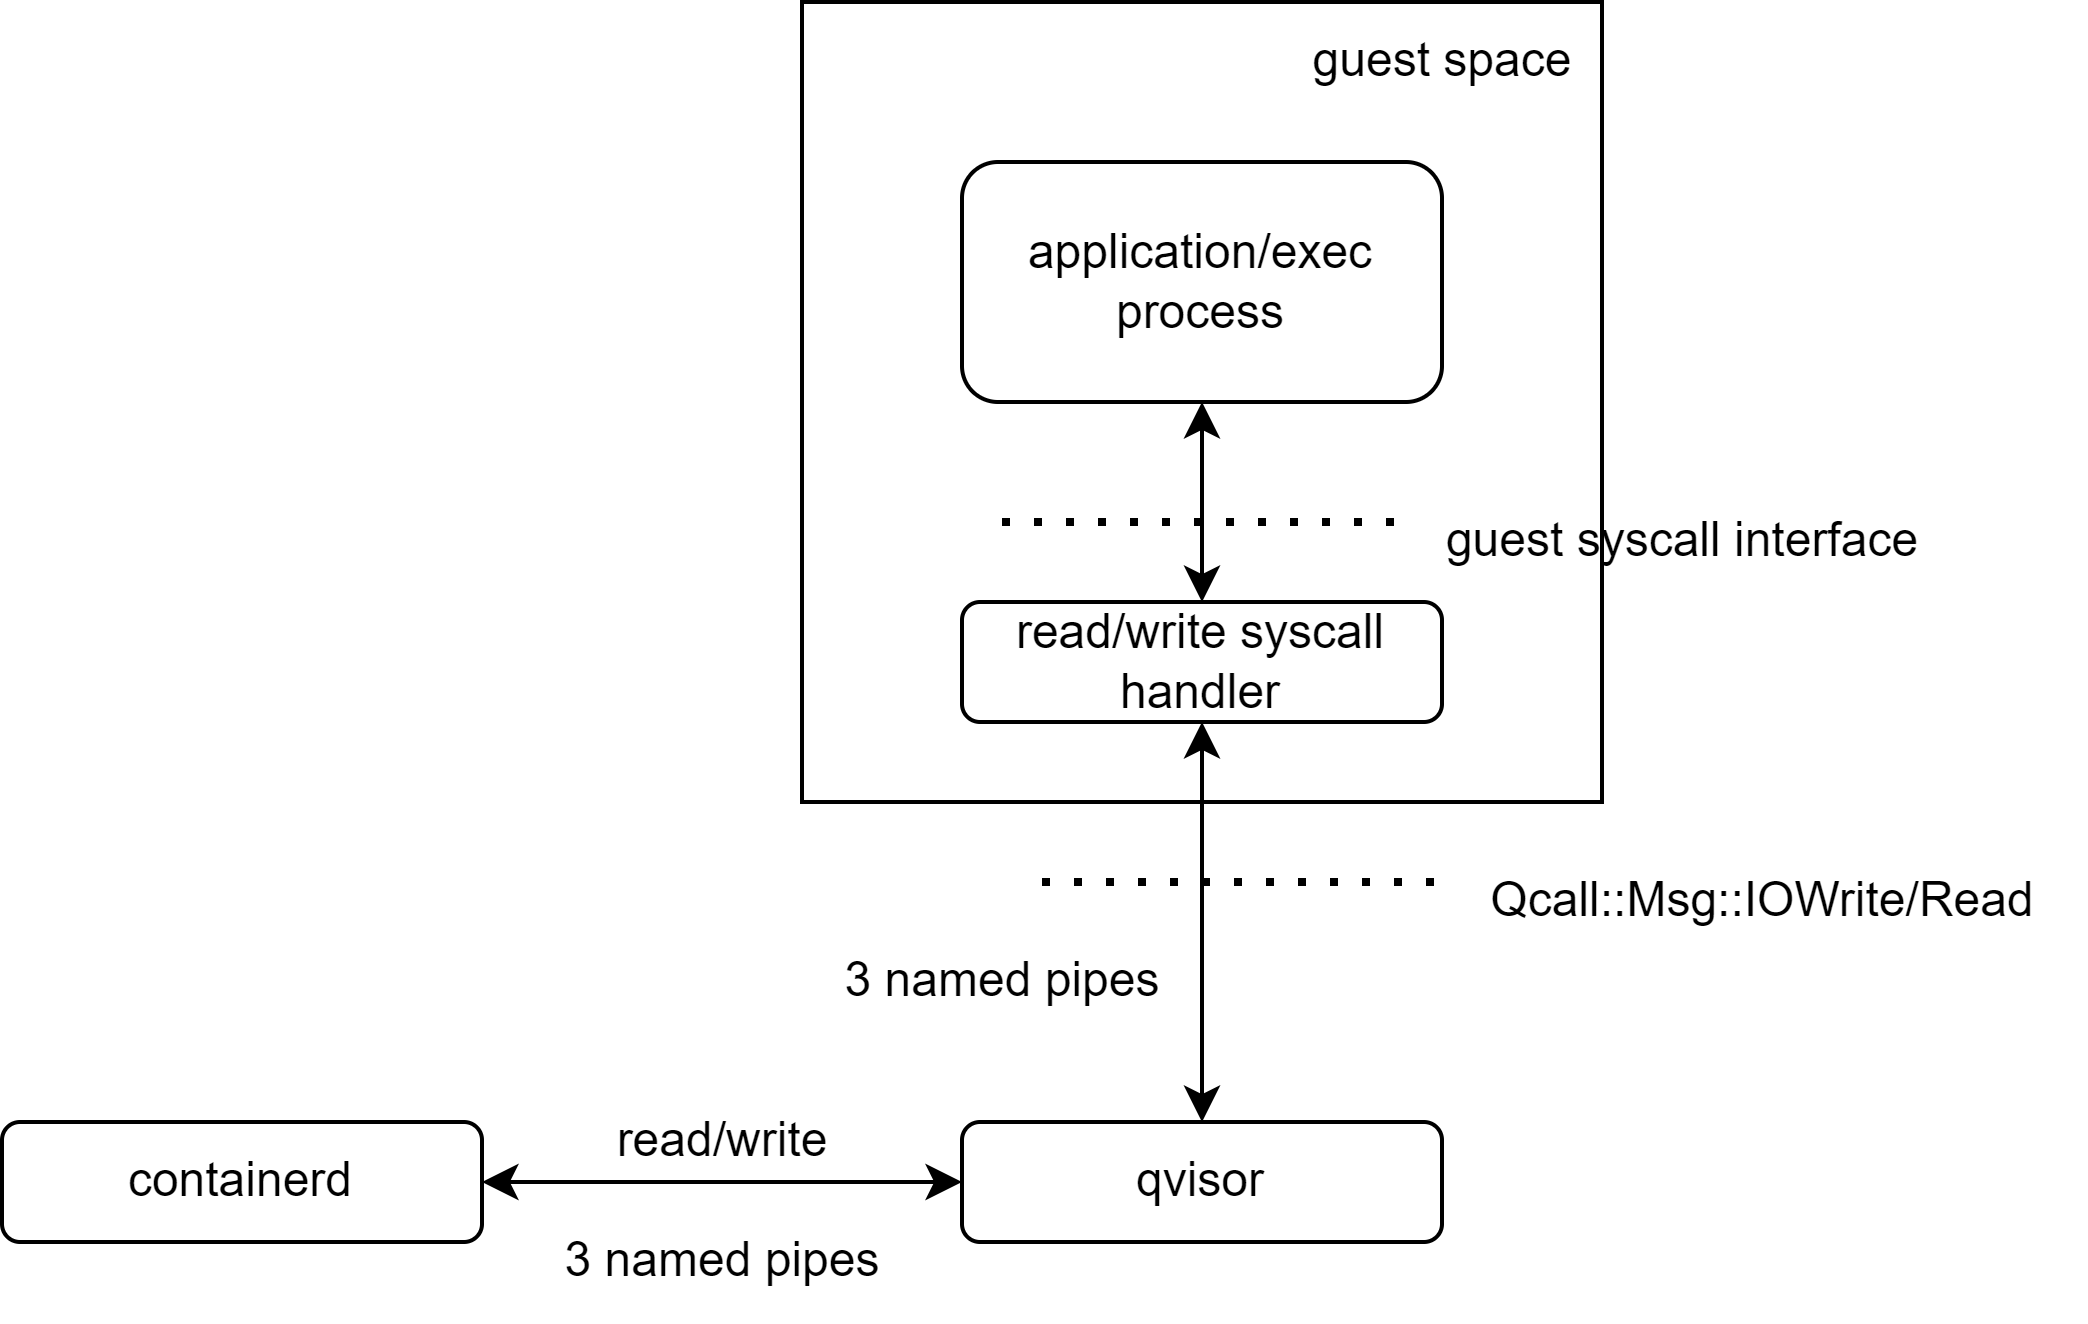
\includegraphics[width=0.8\textwidth]{images/normorl_io.png}
    \caption[Normal STDIO Protection Workflow]{Normal STDIO Protection Workflow}
    \label{fig:normorl_io}
\end{figure}


When it comes to non-interactive applications and EXEC processes, their process's STDIO type falls under Normal IO. In such instances, safeguarding the confidentiality and integrity of data in STDERR and STDOUT of the application and privileged-level 
EXEC processes is vital. To achieve this objective, the Normal STDIO shield utilizes a frame structure that protects the STDOUT and STDERR cryptographically, as shown in Figure~\ref{fig:normorl_io}. This structure includes an encrypted payload, a nonce, and an 
authentication tag. AES-GCM uses the nonce and tag for decryption and authentication. The plaintext payload comprises the information written into STDOUT or STDERR by these processes and a number used to prevent reorder or replay attacks.

Concerning application processes, the number increases sequentially from 0. If a privileged user uses securectl to access an application's logs, this number is utilized to verify whether the log has been reordered or lost. For privileged-level 
EXEC processes, this number is the counter's value in the EXEC request. After receipt of the request's result, securectl compares the reference value and the number in the payload to prevent the replay attack.


\subsection{Terminal STDIO Protection}

\begin{figure}[H]
    \centering
    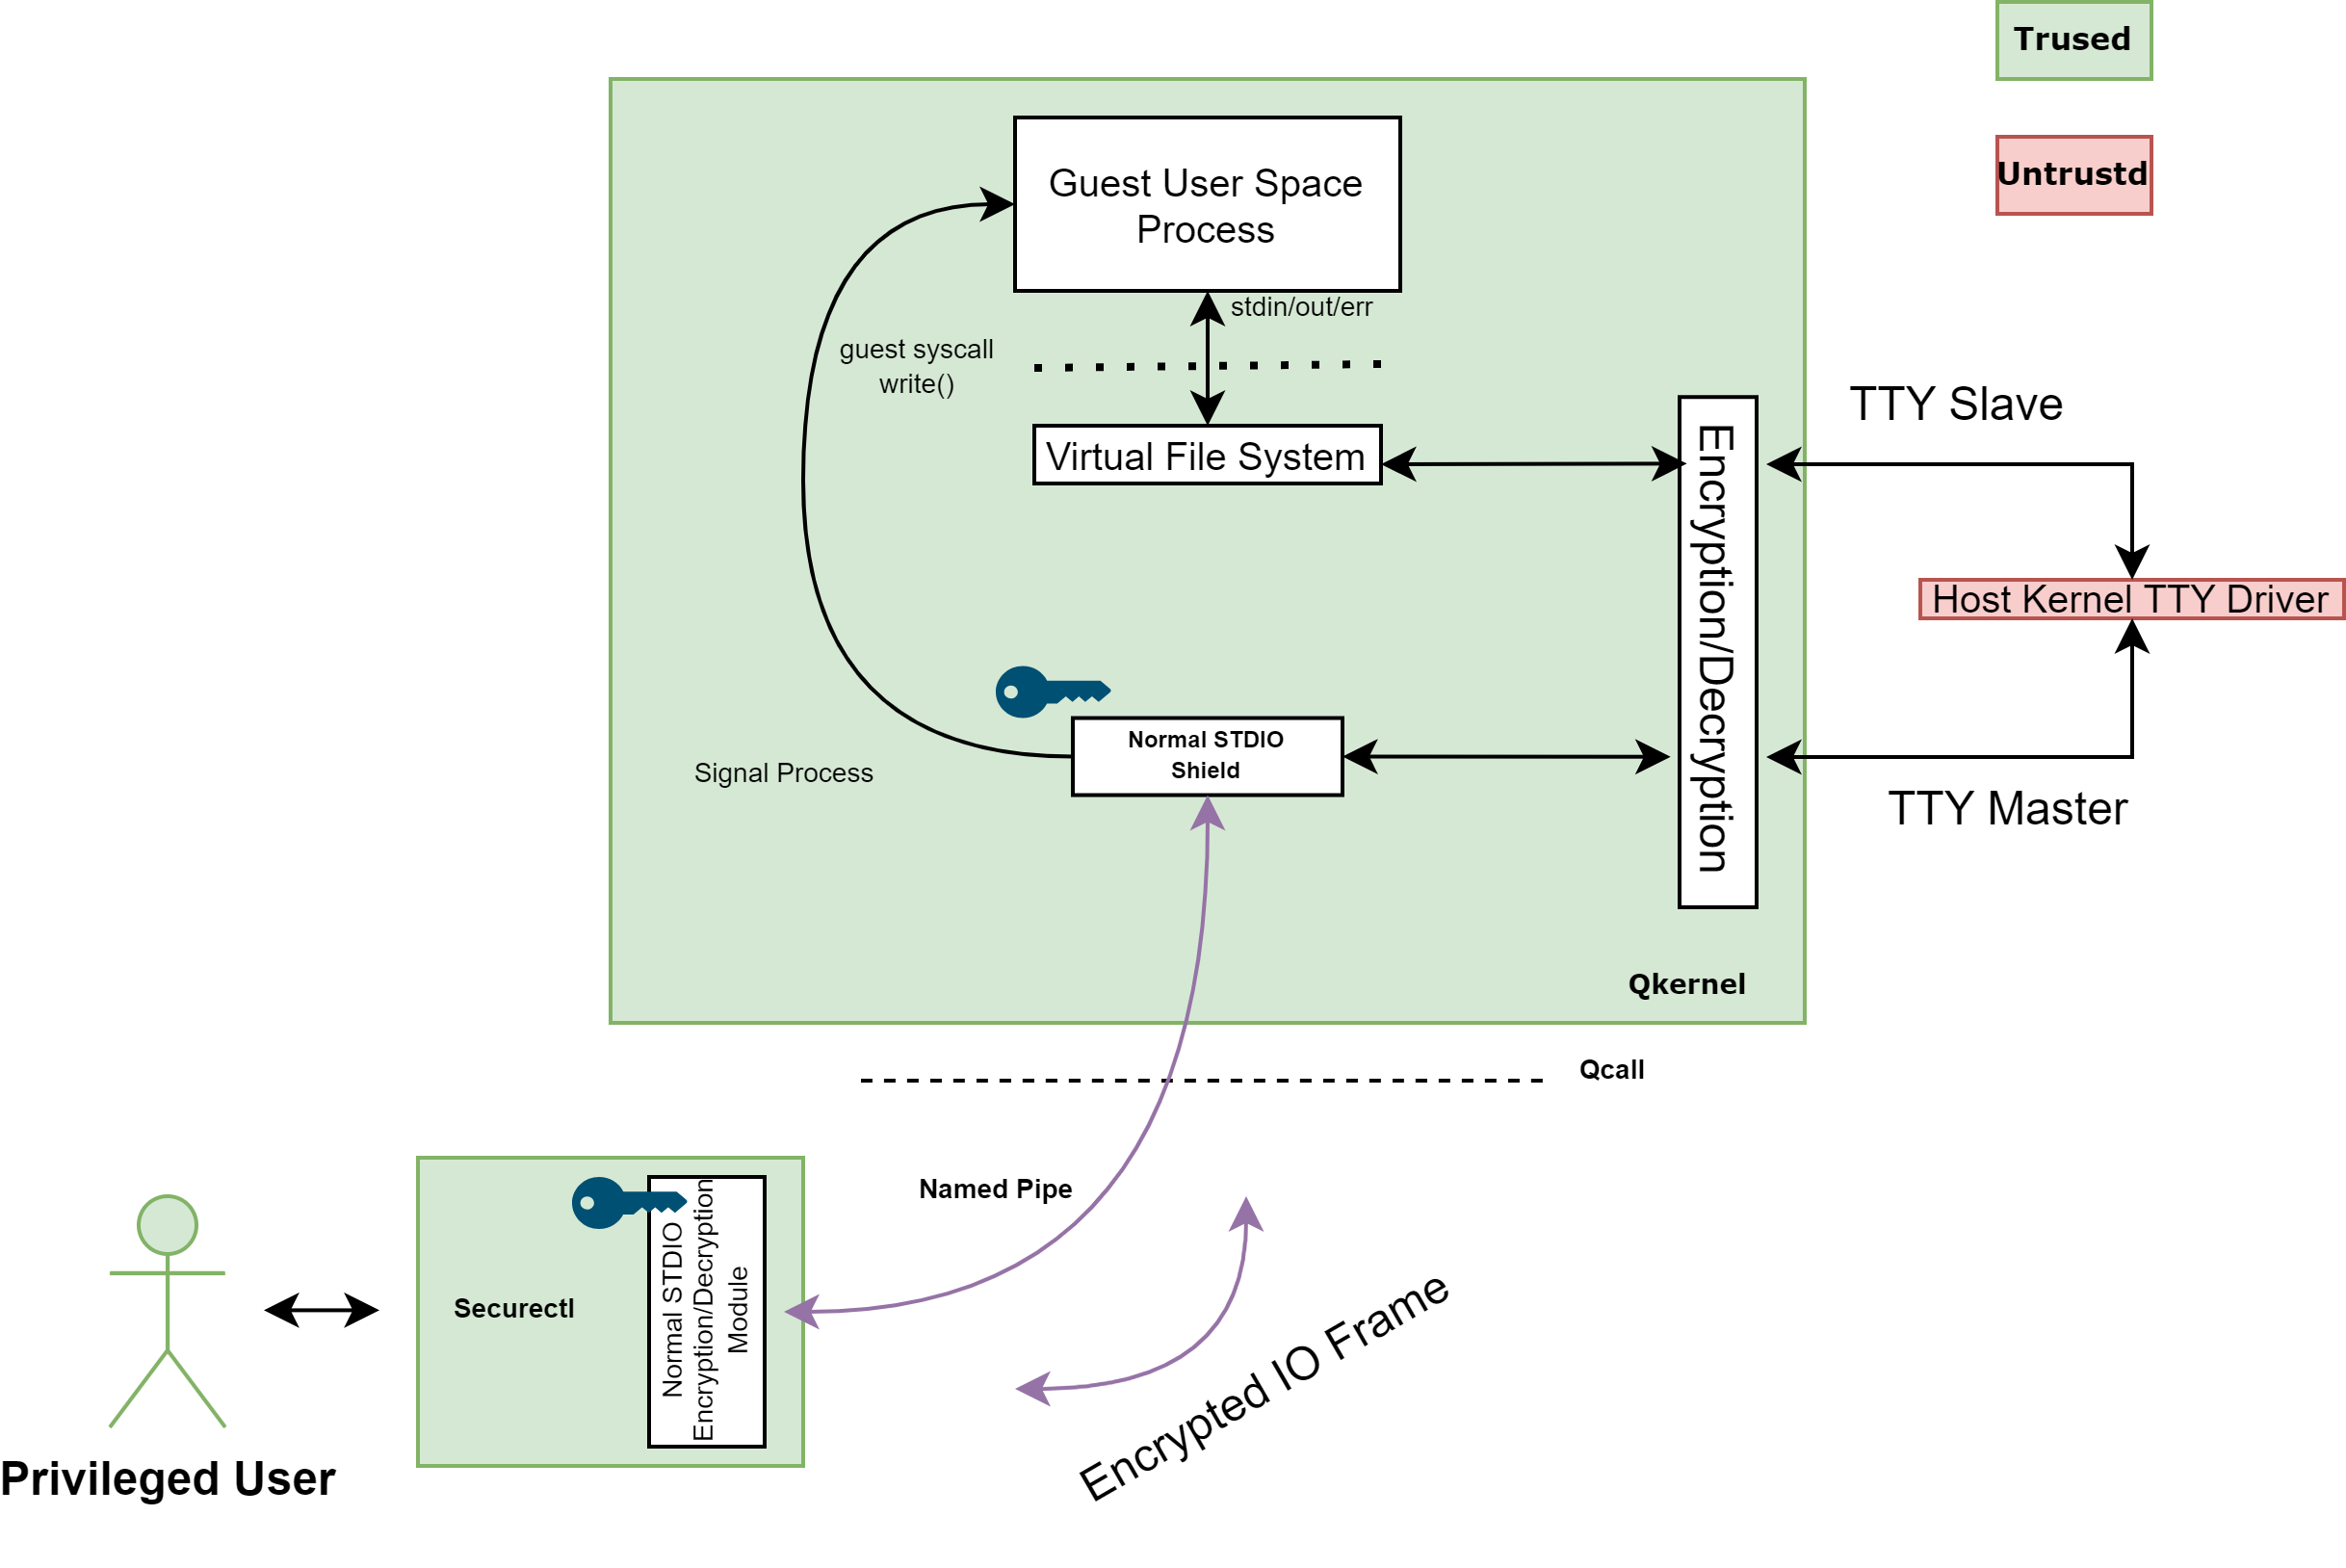
\includegraphics[width=0.6\textwidth]{images/terminal_shiled2.png}
    \caption[Terminal STDIO Protection in case of using Host Kenrel TTY Driver]{Terminal STDIO Protection in case of using Host Kenrel TTY driver}
    \label{fig:terminal_shiled2}
\end{figure}

For interactive applications and EXEC processes, the process's STDIO type is terminal. The goal is to ensure the confidentiality and integrity of data in STDIN, STDOUT, and STDERR of the application and privileged EXEC processes. Achieving this 
requires end-to-end encryption and decryption of the process's STDIO, as shown in Figure~\ref{fig:terminal_shiled2}. This involves encrypting the data written to STDIN on the securectl side and decrypting it in the enclave. STDOUT and STDERR data is encrypted in the enclave and decrypted in the 
securectl. However, implementing end-to-end encryption is complex, as the terminal I/O redirection thread is responsible for filtering the signals from the user and sending them to the enclave. The signals are passed in ASCII code format to the 
thread. When securectl encrypts the data written to STDIN, the redirection thread can no longer filter the signals. To address this issue, the terminal I/O forwarding thread was merged into the normal IO shield in the enclave. Specifically, once 
the encrypted data arrives in the enclave, the Normal IO shield reads the data from the named piped that represents process STDIN, decrypts it, filters out possible signals, and forwards the rest of the data to the tty master.

Since the system still uses the host kernel tty driver, everything written to the tty driver must be encrypted. This affects the enclave's performance. Furthermore, the tty driver's inability to process encrypted data will result in the terminal 
failing to work. For data written to the tty slave, the tty driver needs to translate each line feed (\textbackslash n) into a carriage return followed by a line feed (\textbackslash r\textbackslash n). This editing is required because the user-side terminal needs these two characters 
to start a new line of text. Also, for data written to the tty master, the tty driver will buffer it. Only when the user presses the enter key (\textbackslash r) it copies the buffered data to the tty slave. Since all data written to the tty driver is encrypted, 
it cannot process the data anymore.

\begin{figure}[H]
    \centering
    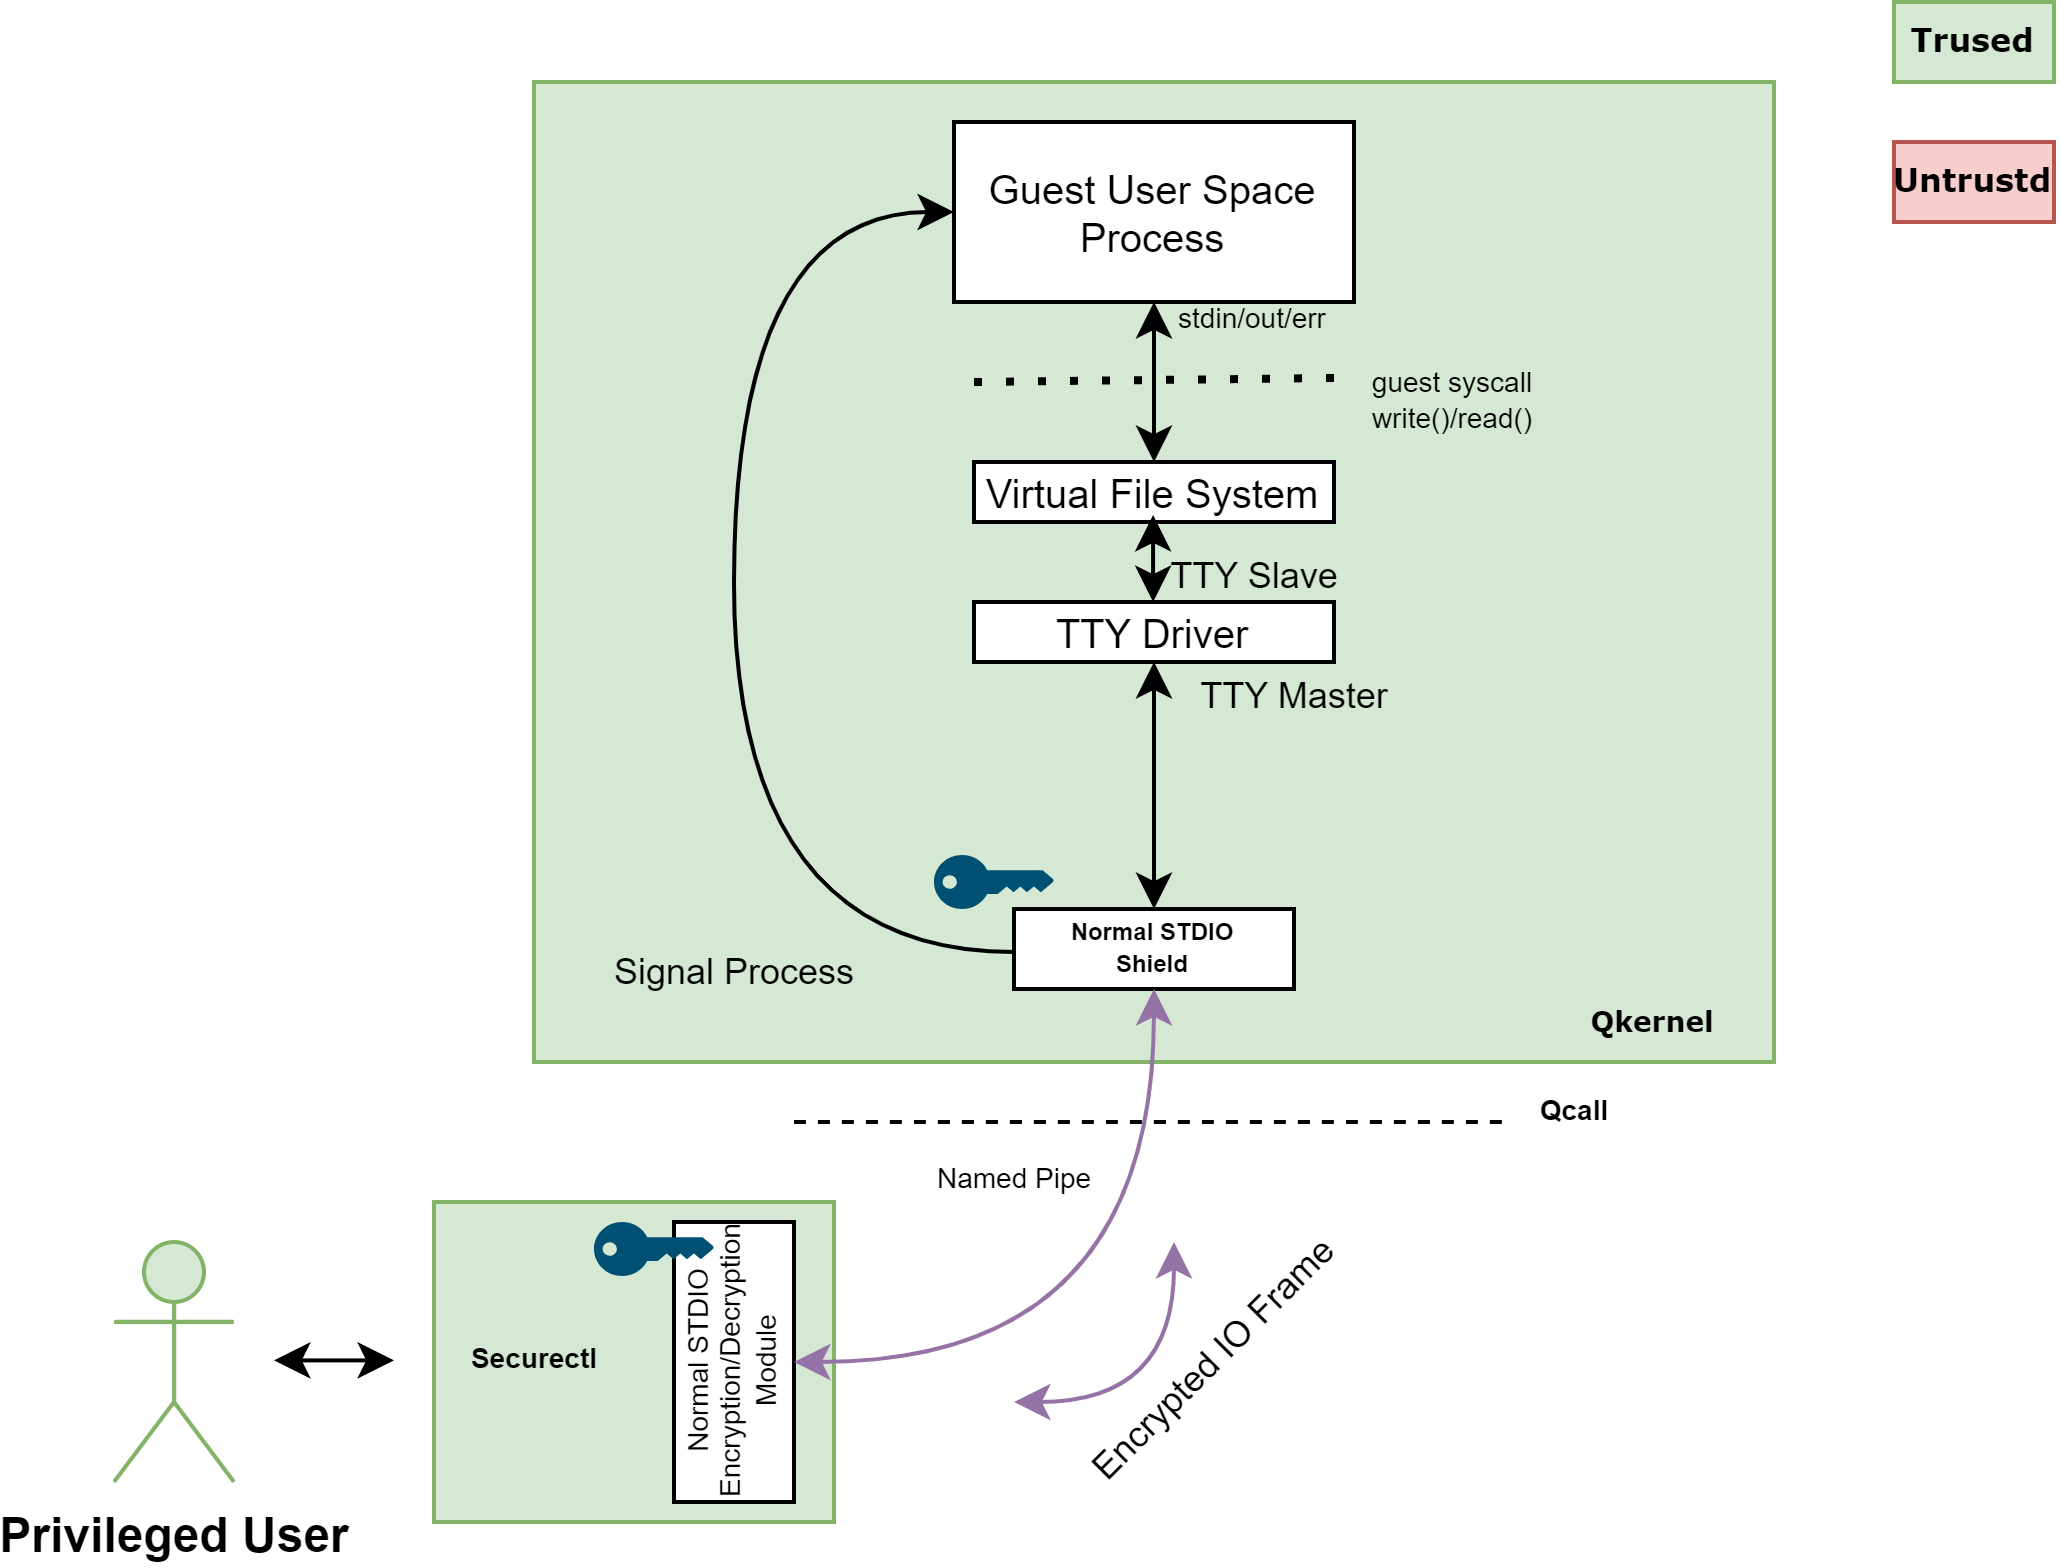
\includegraphics[width=0.8\textwidth]{images/terminal_shiled3.png}
    \caption[Terminal STDIO Protection in case of using Qkernel TTY driver]{Terminal STDIO Protection in case of Qkernel TTY driver}
    \label{fig:terminal_shiled3}
\end{figure}

To resolve this, as shown in Figure~\ref{fig:terminal_shiled3}, a tty driver with functionality similar to the host kernel tty driver has to be implemented in the enclave. This tty driver will be responsible for character echoing, translating between line feeds and carriage returns, and buffering 
the data written to the tty master. When a guest user-space process writes to its STDOUT, the write system call handler redirects the data to a tty slave. The tty driver processes the data, sends it to the tty master, and then notifies the shielding 
layer to start processing it. The shielding layer encrypts the data read from the tty master and sends it to Securectl via the Qcall interface. Securectl then decrypts the data and sends it to the user.

Note that this design has yet to be implemented due to its complexity. As such, it poses two issues. First, the logs of the interactive application are in plaintext, and second, anyone can use kubectl attach -it to connect to the interactive 
application and issue commands. Therefore, as a temporary mitigation, the data written to the STDOUT and STDERR of the interactive application process is encrypted. In this case, the shielding layer encrypts the data before writing it to tty slave 
using ucall, ensuring that the application logs flowing from the interactive application STDOUT or STDERR are encrypted. Although an attacker can connect to the application and issue commands using kubectl attach -it, they will not obtain any 
valuable information because the results returned by the application are encrypted.

\section{System Call Interceptor}
\label{sec:design_Interceptor}
To control the available system calls for guest user space processes, we implemented a system call interceptor in the Qkernel, as illustrated in Figure~\ref{fig:syscall_interceptor}. When a process calls a system call, the CPU jumps to the guest system call entry point. 
This entry point is responsible for finding the system call handler in the Qkernel based on the system call ID. However, before it does so, it must call the interceptor. Based on the shielding layer's policy, the interceptor decides whether the 
system call is allowed. If the system call is not permitted, the guest system call entry point returns EPERM directly to the user state process instead of calling the system call handler.

\begin{figure}[H]
    \centering
    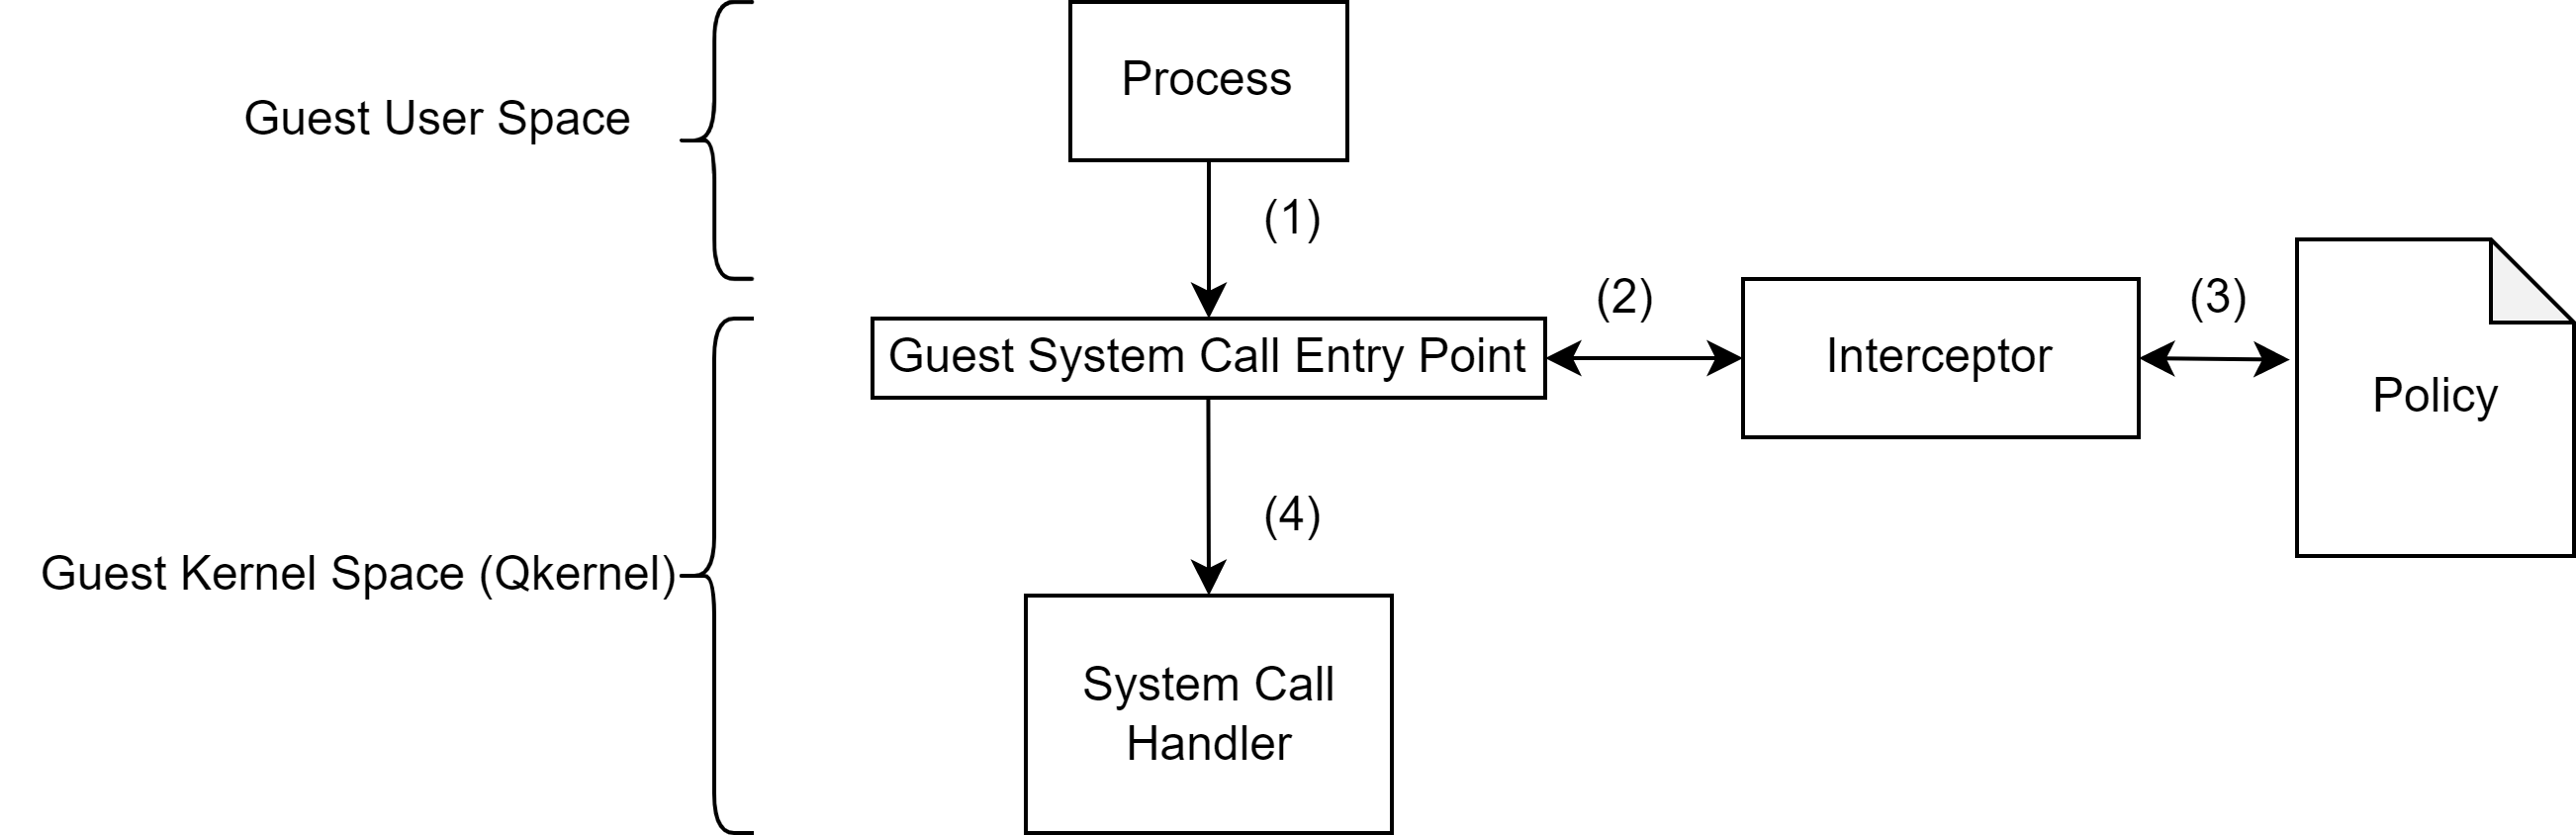
\includegraphics[width=0.8\textwidth]{images/syscall_interceptor.png}
    \caption[System Call Interceptor Workflow]{System Call Interceptor Workflow}
    \label{fig:syscall_interceptor}
\end{figure}

The interceptor policy is displayed in Figure~\ref{fig:policy_system_call}. The application owner can turn the interceptor on or off using the keyword enable. The keyword mode determines the system interceptor's mode, which can be ContextBased or GlobalBased. When the system 
interceptor mode is GlobalBased, it is valid for all guest processes. On the other hand, if ContextBased is enabled, the system interceptor only works for the application process. This is possible because the system interceptor records the 
application process's ID. Considering that there may be multiple processes in the guest user space, such as application processes and EXEC processes. It is strongly recommended that the application owner use the mode GlobalBased. Currently, the 
system interceptor supports only one action, ScmpActErrno, i.e., when the triggered system call's ID is not in the allowlist called syscalls, the system call will be rejected
\begin{figure}[H]
    \centering
    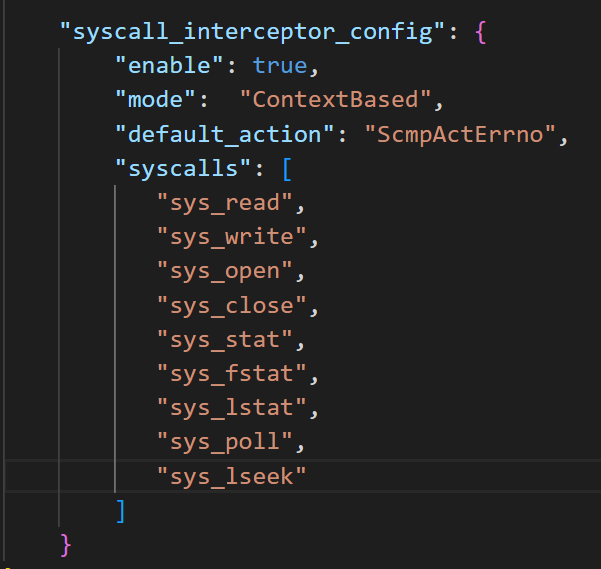
\includegraphics[scale=0.3]{images/policy_system_call.png}
    \caption[System Call Interceptor's Configuration in Shielding Layer Policy]{System Call Interceptor's Configuration in Shielding Layer Policy}
    \label{fig:policy_system_call}
\end{figure}

\section{Qkernel Log Manager}
\label{sec:Qkernel_logger}
Section~\ref{sec:Qkernel_Log_Misconfiguration} of the security analysis discussed the consequences of misconfiguring the Qkernel logging system. Currently, Quark uses a global file to configure the Qkernel and Qvisor. Users can set the logging levels for both using the keyword 
"LogLevel" in this file. Quark supports five logging levels: OFF, ERROR, INFO, DEBUG, and TRACE, where OFF means shutting down the logging system (minimum logging level) and TRACE means printing the most detailed log (maximum logging level). 
Since Qkernel and Qvisor use the same file to configure logging levels, the logging levels are the same for both. However, in confidential computing, Qkernel and Qvisor belong to the application owner and the cloud operator, respectively. They 
have different interests and do not trust each other. For example, to resolve errors quickly, the cloud operator requires the log level in Qvisor to be set to TRACE, while the application owner requires the log level in Qkernel to be OFF (does 
not print any logs) to protect the confidential information in the enclave. In the current architecture, Quark cannot satisfy both requirements.

\begin{figure}[H]
    \centering
    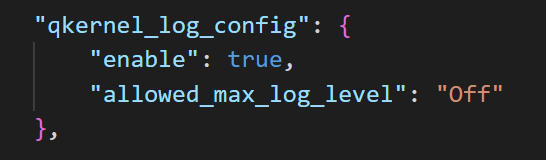
\includegraphics[width=0.8\textwidth]{images/qkernel_Log_config.png}
    \caption[Qkernel Log Configuration in Shielding Layer Policy]{Qkernel Log Configuration in Shielding Layer Policy}
    \label{fig:qkernel_Log_config}
\end{figure}

For this reason, we offload the configuration of the Qkernel logging system from the global configuration file. As shown in Figure~\ref{fig:qkernel_Log_config}, the application owner can configure the Qkernel logging system in the enclave policy. This configuration consists 
of two keywords, enabled and allowed\_max\_log\_level. The keyword allowed\_max\_log\_level represents the maximum log level that the Qkernel can print. For example, when allowed\_max\_log\_level is the INFO, Qkernel only prints logs with the level INFO, 
ERROR. When the keyword ENABLE is false, the Qkernel logging system will use the default log level from the global file. In addition, enclave policy is passed to the enclave during application deployment. Before the enclave gets the policy, the 
enclave uses the default log level OFF.


\section{Modification to OCI}

\subsection{Extending the container lifecycle to support confidential computing}
The container lifecycle definition in the OCI RUNTIME specification~\cite*{oci-runtime-spec} lacks support for remote attestation and the protection for application’s STDIO. In confidential computing, the relying party uses the remote 
attestation mechanism to verify the user-specified program and supply it with secrets. The types of secrets include environment variables, command line arguments, and files. Also, as known from Chapter~\ref*{sec:security_analyse}, the application 
process STDIO needs to be protected. In this section we first give the definition of container runtime and enclave in the context of confidential computing. Then we will propose modifications to the container lifecycle


\subsubsection{Definition of Runtime and Enclave in Confidential Computing}

Currently, the container runtime in the OCI runtime specification~\cite*{oci-runtime-spec} refer to a runtime environment used to create containers. For a VM based container runtime, it includes the shim process, the hypervisor, and the components 
inside the guest that are used to create and manage the container. For example, in the kata container, the three components correspond to kata-shim, qemu, and kata-agent, respectively. However, in confidential computing, the guest runs in an 
encrypted virtual machine. This means that the components inside the guest are trusted, while the shim process and hypervisor are not trusted. Therefore, we redefine runtime as untrusted runtime components, e.g., kata-shim and qemu. 
In addition, we refer to the components that run in trusted environments for creating containers as enclaves in general, e.g., kata agent, guest kernel, etc.

\subsubsection{Modification to Container Lifecycle}
We make the following changes to the container lifecycle. Note that the bold text in the list is the part we modified, the rest is copied from OCI RUNTIME SPECIFICATION~\cite*{oci-runtime-spec}.

\begin{enumerate}
    \item OCI compliant runtime's create command is invoked with a reference to the location of the bundle and a unique identifier.
    \item The container's runtime environment and enclave MUST be created according to the configuration in config.json. If the runtime is unable to create the environment specified in the config.json, it MUST generate an error. While the resources requested in the config.json MUST be created, the user-specified program (from process) MUST NOT be run at this time. Any updates to config.json after this step MUST NOT affect the container
    \item The prestart hooks MUST be invoked by the runtime. If any prestart hook fails, the runtime MUST generate an error, stop the container, and continue the lifecycle at step 16
    \item The createRuntime hooks MUST be invoked by the runtime. If any createRuntime hook fails, the runtime MUST generate an error, stop the container, and continue the lifecycle at step 16.
    \item The createContainer hooks MUST be invoked by the runtime. If any createContainer hook fails, the runtime MUST generate an error, stop the container, and continue the lifecycle at step 14.
    \item Runtime's start command is invoked with the unique identifier of the container.
    \item The startContainer hooks MUST be invoked by the runtime. If any startContainer hook fails, the runtime MUST generate an error, stop the container, and continue the lifecycle at step 14.
    \item \textbf{The Enclave receives the runtime’s start request and constructs a process for the user-specified program, as specified by process. If this hook fails, the enclave MUST generate an error, stop the container, and continue the lifecycle at step 16}
    \item \textbf{The enclave Must invoke the application launch measurement hook if the user-specified program’s binary is loaded from the host. If this hook fails, the enclave MUST generate an error, stop the container, and continue the lifecycle at step 16.}
    \item \textbf{The attestation and provisioning hook MUST be invoked within the enclave when the enclave finish loading the program’s binary. If this hook fails, the enclave MUST generate an error, stop the container, and continue the lifecycle at step 16.}
    \item \textbf{The process for the user-specified program enters user space and starts to run.}
    \item \textbf{The enclave MUST invoke the runtime measurement hook when the program process loads binary or shared library from the host. If this hook fails, the enclave MUST generate an error, stop the container, and continue the lifecycle at step 16}
    \item \textbf{The enclave must invoke the STDIO protection hook when the program/exec process reads or writes data from its standard IO. If this hook fails, the enclave MUST generate an error, stop the container, and continue the lifecycle at step 16}
    \item The poststart hooks MUST be invoked by the runtime. If any poststart hook fails, the runtime MUST log a warning, but the remaining hooks and lifecycle continue as if the hook had succeeded.
    \item The container process exits. This MAY happen due to erroring out, exiting, crashing or the runtime's kill operation being invoked.
    \item Runtime's delete command is invoked with the unique identifier of the container.
    \item The container MUST be destroyed by undoing the steps performed during create phase (step 2).
    \item The poststop hooks MUST be invoked by the runtime. If any poststop hook fails, the runtime MUST log a warning, but the remaining hooks and lifecycle continue as if the hook had succeeded.    
  \end{enumerate}


  The application launch measurement hook should be called when the enclave loads the application binary from the host. This hook must be executed in the enclave namespace. It is responsible for measuring the application binaries loaded from the 
  host. The attestation and provisioning hook will send the measurement results to the relying party as part of the attestation report for integrity check. Note that the TEE hardware must measure this hook as part of the enclave container runtime 
  component.
  

  The attestation and provisioning hook must be invoked after the enclave loads the application binary but before the application process stack is set. This hook provides a mechanism for the enclave to authenticate itself to the relying party and 
  retrieve the secret. We recommend that runtime developers implement a KBS Client in the enclave based on the KBS attestation protocol as the remote attestation and provisioning hook. We provide a reference implementation in Chapter 5. Note that 
  this hook must be executed in the enclave namespace. Alternatively, it can be measured by the TEE hardware as part of the enclave container runtime component or loaded by the host as a binary file. In the latter case, the hook must be measured 
  by the application launch measurement hook. If the application binary is loaded from the host, the attestation report the hook sends to the relying party must include the application launch measurement hook's measurement. After the attestation 
  and provisioning hook retrieves the secret, it should push the environment variable and application parameter type secret into the application process's stack. For the file type secret, it should store it within the enclave, and implement a 
  mechanism to make it accessible to the application. We provide a reference implementation in Section 5.
  \todo{add link  in Section 5}

  The runtime measurement hook should by called by the enclave should call  when the application loads a shared library or binary file from the host at runtime. This hook must be executed in the enclave namespace. It measures the shared libraries or 
  binaries loaded from the host at application runtime. It compares the measurement result with the reference value. If the two do not match, the hook execution fails. In this case, the enclave must generate an error, stop the container, and 
  continue the life cycle at step 16. Note that the reference values are obtained by the attestation and provisioning hook from the relying party during application deployment. Alternatively, this hook can be measured by the TEE hardware as part 
  of the enclave container runtime component or as a binary file loaded from the host at application startup. In the latter case, this hook must be measured by the application launch measurement hook.
  

  The STDIO protection hook should be called when the application process or privileged exec process reads or writes its STDIO. This hook is responsible for cryptographically protecting the STDOUT and STDERR of the process. It is also responsible 
  for decrypting the data read from stdin when the STDIO type of the process is terminal. A reference can be found in Section~\ref*{sec:design_STDIO_PROTECTION} . Alternatively, this hook can be measured by the TEE hardware as part of the enclave container runtime 
  component or as a binary loaded from the host at application startup. In the latter case, this hook must be measured by the application launch measurement hook.
  
\subsection{EXEC Operating Guidelines}

  There was much discussion in the OCI Runtime spec community about the semantics of EXEC operations. Ultimately, however, the runtime spec decided not to standardize on EXEC operations~\cite*{exec_semantics}. This gives runtime developers more freedom to implement it 
  according to their specific needs. However, in a confidential computing scenario, EXEC opens a backdoor for attackers to steal an application’s secrets running in an Enclave. For this reason, we propose a standardized EXEC operation for the 
  confidential computing scenario.

  We use the proposal for standardizing EXEC operations in Figure~\ref{fig:exec_propose} as a starting point. This proposal was submitted to the OCI Runtime spec forum, but ultimately was not adopted for the reasons mentioned earlier.

\begin{figure}[H]
    \centering
    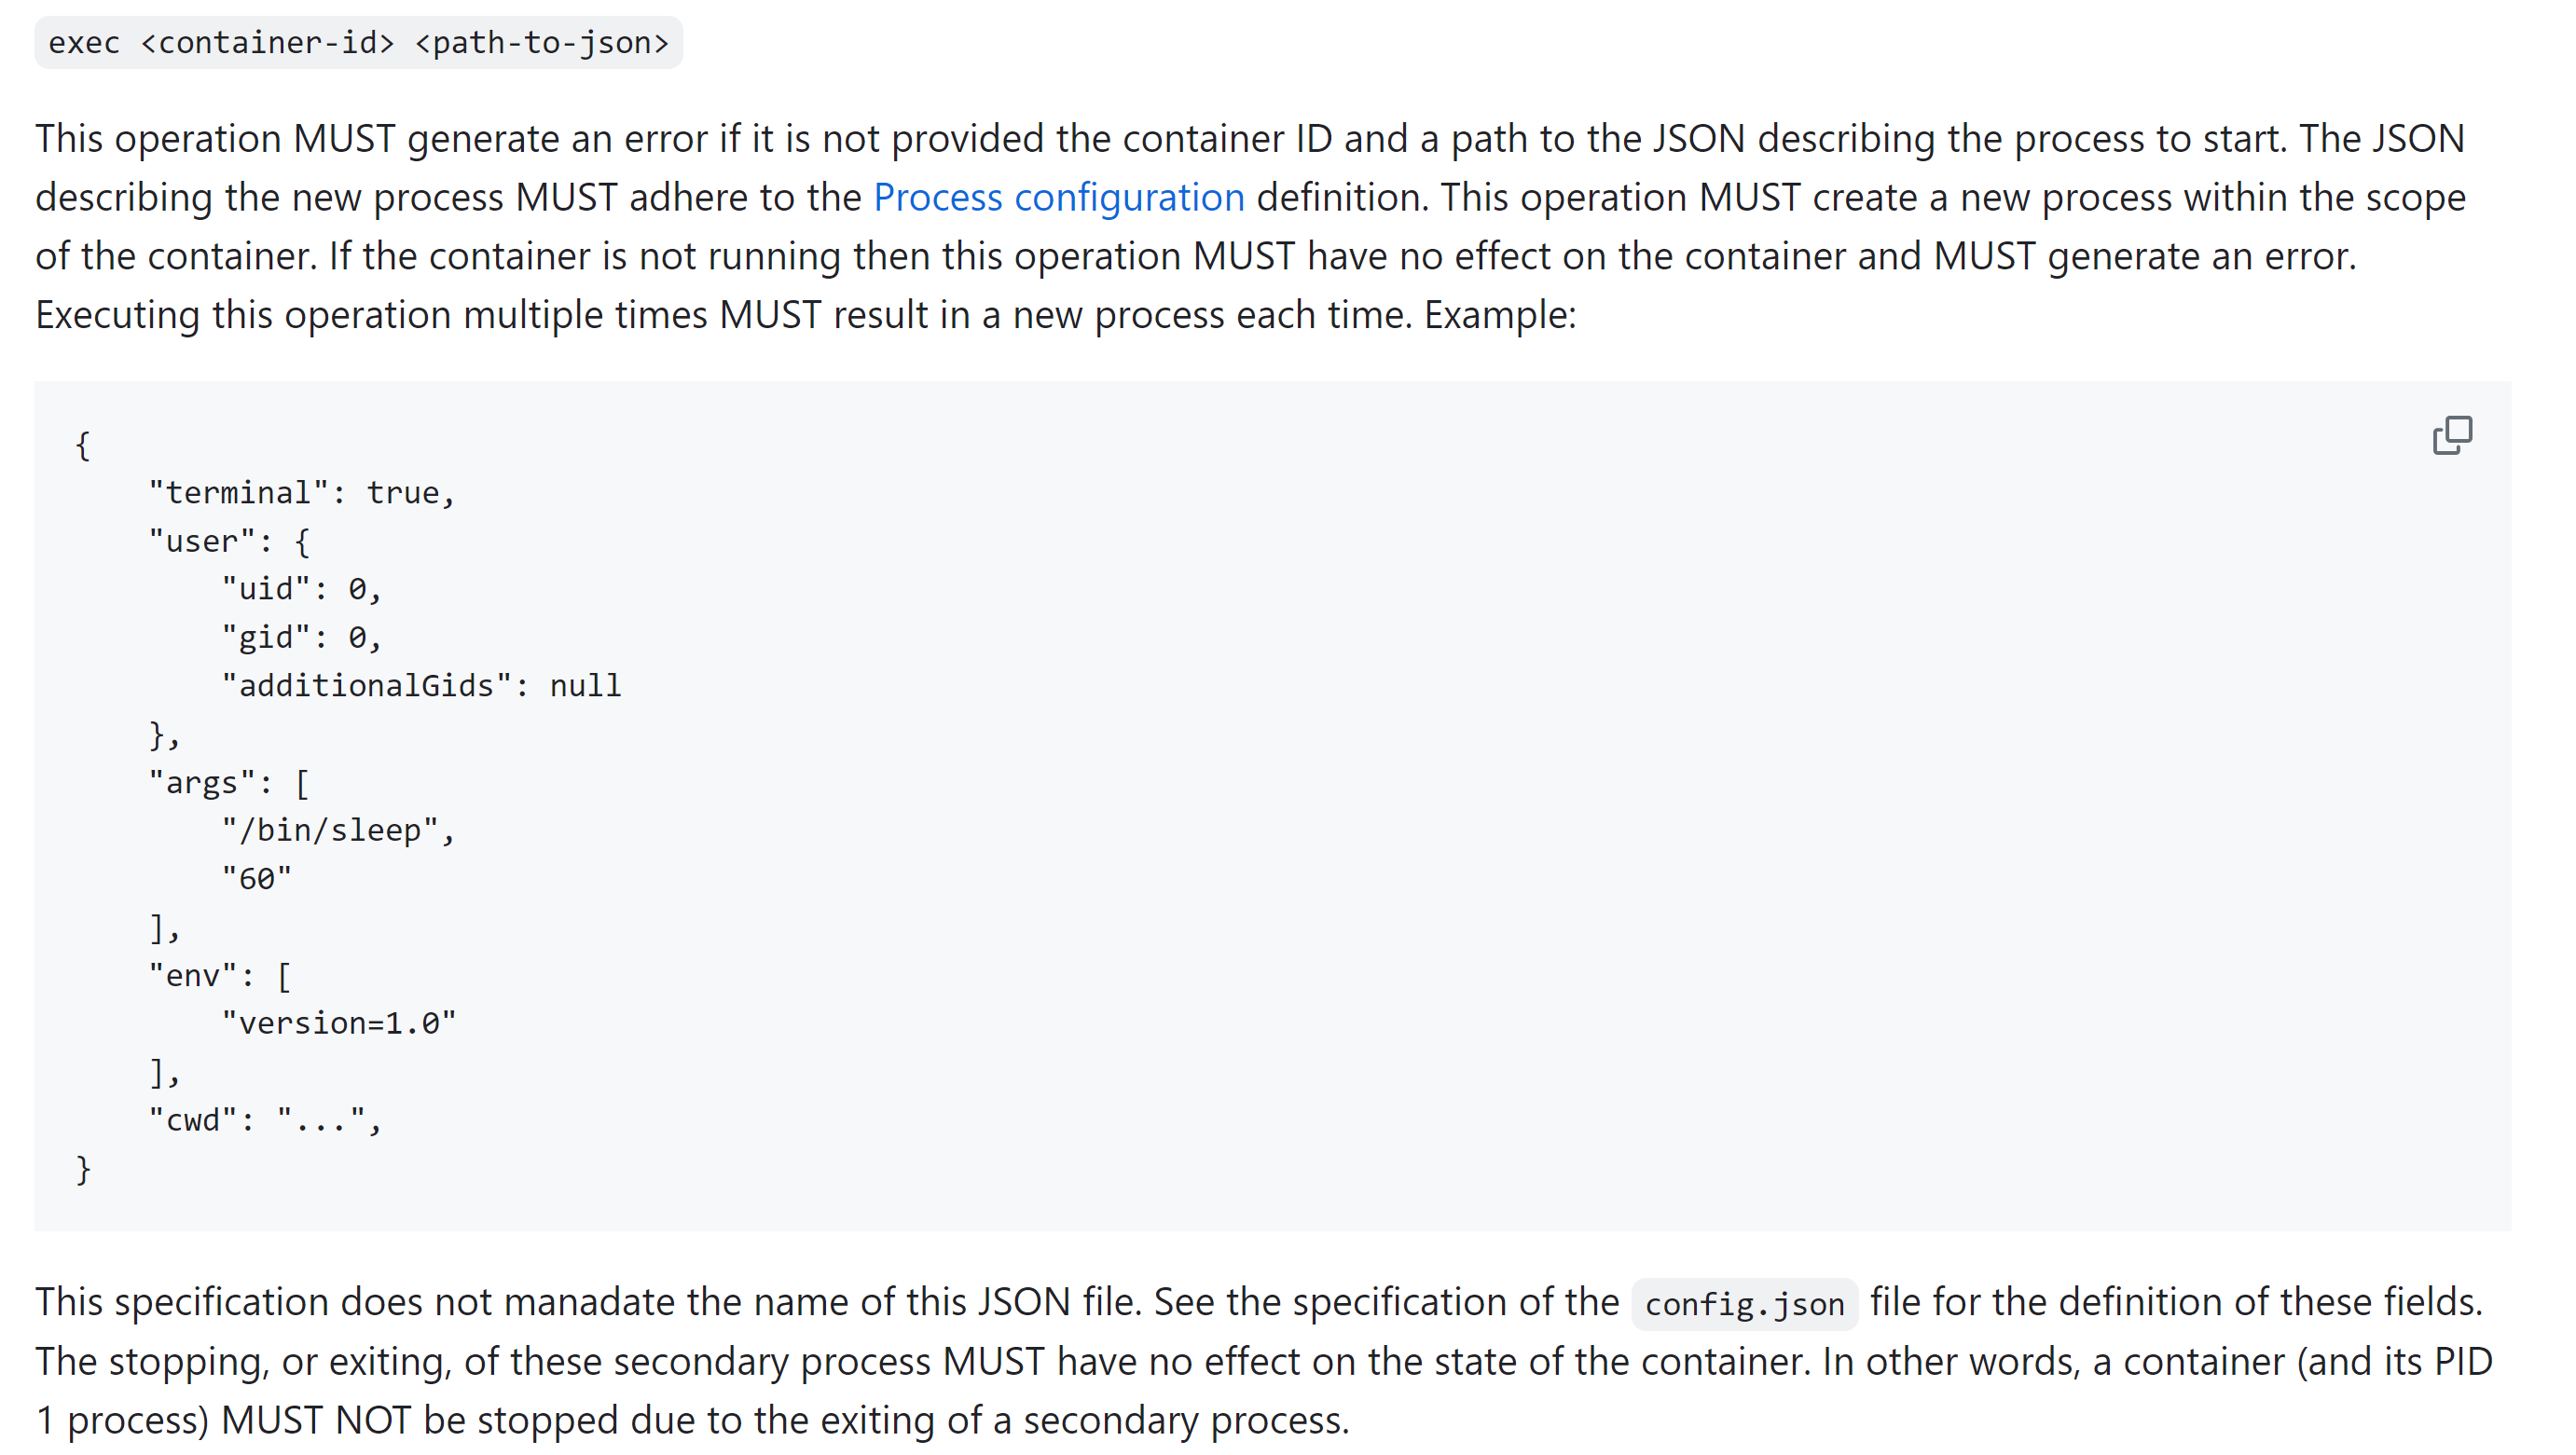
\includegraphics[width=0.8\textwidth]{images/exec_propose.png}
    \caption[Proposal for standardizing EXEC operation]{Proposal for standardizing EXEC Operation from~\cite*{exec_proposal} }
    \label{fig:exec_propose}
\end{figure}


  In a confidential computing scenario, exec requests should be divided into two categories, namely privileged  request issued by the application owner and unprivileged requests issued by otherss. We have 2 goals here. First, we want to restrict 
  the commands that users at each privilege can issue to the application following the least privilege principle. Second, we want to protect the commands issued by privileged-level users and its execution results. Therefore, the args in the json file 
  of privileged EXEC requests must be protected. The protection mechanism is discussed in Figure~\ref{fig:new_pattern_of_exec} and in Section~\ref{sec:design_EXEC_Requests}. This mechanism effectively distinguishes between privileged and unprivileged requests and ensures the confidentiality, integrity, 
  and authenticity of commands issued by privileged users. The enclave should authenticate and access control the request before creating the EXEC process. The authentication is done by using a key shared between the privileged user and the enclave. 
  This key is fetch by the attestation and provisioning hook from relying party. The steps for access control are as follows. First the enclave determines the type of the EXEC request by checking if the first element in the args array is Privileged. 
  It then reads the policy and determines whether this command is allowed to be executed. The content of the policy is shown in Figure~\ref{fig:exec_policy}. In particular, the policy is  obtained by the attestation and provisioning hook.  
  The policy specifies the commands that can be executed by users at each privilege and the directories in which these commands has access to. We will provide a reference algorithm for the access control in Chapter 4.
  \todo{add link Chapter 4}

  In addition, to protect the results of privileged-level EXEC requests, the enclave must encrypt the stdout and stderr of privileged-level processes. The encryption mechanism can be found in Section~\ref{sec:design_STDIO_PROTECTION}.
  

\section{Summary}
In this chapter, we present mechanisms for protecting the integrity and confidentiality of a secure application's secrets when it is orchestrated by untrusted k8s. We demonstrate a secure approach to deploying applications, and how to protect 
the confidentiality and integrity of the application's standard flows, restrict the commands users can issue to the application, and propose modifications to the OCI interface. With these approach, applications can be orchestrated in a secure 
manner by untrusted entities. In next chapter, we describe how we implemented this mechanisms .
\cleardoublepage

%%% Local Variables:
%%% TeX-master: "diplom"
%%% End:
